\documentclass[english,master]{unibg}


\usepackage{todonotes}
\usepackage{listings}
\usepackage{xcolor}


\newlength\dunder
\settowidth{\dunder}{\_}
\newcommand{\twound}{\rule{2\dunder}{0.4pt}}


\definecolor{codegreen}{rgb}{0,0.6,0}
\definecolor{codegray}{rgb}{0.5,0.5,0.5}
\definecolor{codepurple}{rgb}{0.58,0,0.82}
\definecolor{backcolour}{rgb}{0.95,0.95,0.92}

\lstdefinestyle{mystyle}{
	backgroundcolor=\color{backcolour},   
	commentstyle=\color{codegreen},
	keywordstyle=\color{magenta},
	numberstyle=\tiny\color{codegray},
	stringstyle=\color{codepurple},
	basicstyle=\ttfamily\footnotesize,
	breakatwhitespace=false,         
	breaklines=true,                 
	captionpos=b,                    
	keepspaces=true,                 
	numbers=left,                    
	numbersep=5pt,                  
	showspaces=false,                
	showstringspaces=false,
	showtabs=false,                  
	tabsize=2
}

\lstset{style=mystyle}


\title{Exploring eBPF for Windows}
\subtitle{Implementation analysis and comparison with Linux}
\advisor{Chiar.mo Prof.~Stefano Paraboschi}
% \coadvisor{Chiar.mo Prof.~Ed Smith}

\department{Ingegneria Gestionale, dell'Informazione e della Produzione}
\course{Ingegneria Informatica}
\class{LM-32}

\author{Matteo Locatelli}
\studentid{1059210}
\academicyear{2022/2023}

\begin{document}
\maketitle
\emptypage

\begin{abstract}

\textit{Berkeley Packet Filter} (\textit{BPF}), an originally Unix-based packet filtering technology, has evolved into a versatile tool with significant impact on network performance and security. 
This master thesis aims to explore the story of BPF, tracing its development from its inception on Unix-based systems to its adaptation on Windows platforms. 
Through a comparative analysis, we investigate the challenges, solutions and advancements that have led to the successful integration of BPF in the Windows environment. 
By studying its history, architecture and 
programs development, we explore the potential of BPF to revolutionize network engineering on Windows and contribute to the broader understanding of cross-platform technology adoption.

\end{abstract}

\emptypage

\section*{Acknowledgements}

Completing this master thesis on the evolution and adaptation of Berkeley Packet Filter on both Linux and Windows platforms has been an enriching journey for me. 
I am deeply grateful to the individuals whose guidance, encouragement and support have made this research possible. 
Without their firm belief in my abilities, this effort would not have come to completion.

First and foremost, I extend my heartfelt gratitude to my esteemed advisor, professor Stefano Paraboschi, whose expertise, mentorship and invaluable feedback have been instrumental in shaping this thesis. 

My sincere appreciation must be extended to the people in the \textit{Unibg Security Lab} \cite{UnibgSeclabWebsite} team who actively participated in the development of this thesis: their continuous support throughout the entire research process have motivated me to push my boundaries and aim for excellence. 
I am grateful for their patience, insightful discussions and profound knowledge in the fields of computer engineering and systems security, which have significantly contributed to the depth and quality of this work: their willingness to share their expertise has been essential in overcoming various challenges faced during this study and in refining the ideas presented in this research.
Their support has made this academic pursuit not only a productive venture, but also an enjoyable one.
Also, they provided me with the LaTex template that I used to write this thesis.

Speaking of people that gave me something practical that helped me to work on this project, I have to thank Subconscious Compute \cite{SubComWebsite}, an Indian IT company founded in 2020 that works on security for distributed devices and data.
Their decision to open-source their GitHub repository, which is under AGPL license, and grant me access to it has been fundamental in enabling me to develop eBPF programs on the Windows platform and to do a better comparison with eBPF on Linux, which was the scope of my master's thesis.
The availability of the repository not only provided me with a lot of resources and code examples, but also allowed me to gain insights into best practices and advanced techniques in programming for Windows using eBPF. 

Moreover, I would like to express my obligation to the wider academic community of the \textit{Università degli Studi di Bergamo} \cite{UnibgWebsite} for providing an environment that encourages learning, curiosity and innovation. 
I am deeply grateful to everyone who played a part, big or small, in the ending of my academic journey. 
The education I received has been invaluable and I am fortunate to have had such exceptional guidance throughout my academic period. 
This thesis stands as a testament to the collective effort and support of those who have been part of my academic journey. 
The knowledge and experiences I have gained throughout the last five years have been instrumental in shaping my growth as a computer engineering student.

Last but not least, I must express my very profound gratitude to my parents for their love, encouragement and support throughout eighteen years of education. 
Their belief in my capabilities and constant motivation have been the driving force of my academic achievements, especially during the demanding period of writing this thesis.
I owe my successes to them because with their sacrifices they have allowed me to focus on my studies and achieve my academic goals, celebrating every milestone with infinite joy and pride.
In conclusion, I am grateful for the life lessons and values they instilled in me, which have shaped me into the person I am today.

Thank you.

\toc[figures,tables,listings]
\emptypage

\clearpage
\pagenumbering{arabic}

% https://ebpf.io/ -> COMMUNITY TALKS FOR DEEPER INSIGHTS

\chapter{Introduction}

In the ever-evolving landscape of computer science and networking, the demand for efficient, flexible and secure packet filtering technologies has been dominant. 
The \textit{Berkeley Packet Filter} (\textit{BPF}), an innovative technology developed in the Unix environment, has emerged as a powerful tool for network monitoring, traffic analysis and security enforcement. 
Over the years, BPF has undergone significant advancements, culminating in the birth of \textit{Extended Berkeley Packet Filter} (\textit{eBPF}), a groundbreaking extension that has revolutionized network engineering and performance analysis.

\section{Background}

Computer networks establish the backbone of modern communication, enabling the consistent exchange of information across the globe. 

The rapid growth of network traffic, the rise of complex cyber threats and the increasing need for real-time monitoring have motivated researchers and engineers to explore innovative solutions to enhance network performance and to build robust security mechanisms.
Packet filtering, a fundamental networking technique, serves as a first line of defense in safeguarding networks and optimizing data transmission.

Originally conceived in the 1990s, the Berkeley Packet Filter was designed as a mechanism to filter packets at the kernel level for the \textit{Berkeley Software Distribution} (\textit{BSD}) operating system, a discontinued operating system based on the early versions of Unix. 
However, its potential, consisting of its lightweight and versatile design, far exceeded its initial purpose and it evolved into a versatile technology with applications across various networking domains.

Over the years, BPF has undergone significant developments and adaptations, until it resulted in the advent of eBPF: with the introduction of a new virtual machine and bytecode, eBPF allowed for the dynamic execution of custom programs within the kernel context, extending its applicability beyond traditional packet filtering to areas such as network monitoring, tracing and deep packet inspection.

\section{Motivation}

Despite the extensive use of eBPF in Unix-based systems, its incorporation into Windows environments has remained a challenge. 
As Windows continues to be a prominent operating system in both personal and enterprise computing, unlocking the potential of eBPF on this platform becomes crucial for achieving cross-platform network engineering and security solutions.

This thesis will focus on the historical progression of BPF and its adaptation on the Windows platform.
In addition to that, we will explore the advancements introduced to eBPF on both operative systems and study the current state of art of eBPF on Windows to show its differences with the Linux environment. 

\section{Objectives}

This master's thesis aims to provide an in-depth analysis of eBPF's architecture, installation and functionality in both operating systems, while showing the history, development and impact of eBPF in the world of computer science and network engineering. 

The primary objectives of this research are as follows:

\begin{itemize}
	\item 
		Tell the history of eBPF: by understanding the origins of BPF, we gain insights into the motivations that led to the creation of eBPF and we can identify the key challenges faced during its integration into Windows and the innovative solutions designed to overcome them. 
		A look into the historical context provides a solid foundation for exploring eBPF's potential, from a simple packet filtering mechanism to a versatile technology with broader network real-world applications;
	\item 
		Installation and integration of eBPF on Linux and Windows: we will investigate the process of installing eBPF into both Linux and Windows operating systems. 
		By understanding the differences in installation procedure and requirements on these platforms, we are enabled to leverage the cross-platform capabilities of this technology;
	\item 
		Development of eBPF programs on Linux and Windows: this thesis will cover the development process of eBPF programs on both Linux and Windows platforms. 
		We will explore the process of creating, loading and executing eBPF programs.
		Furthermore, by studying the eBPF API, we will:
		\begin{itemize}
			\item 
				Demonstrate the creation of custom programs to achieve specific networking tasks;
			\item 
				Show how far they have come in the development of the technology in the two operating systems;
			\item 
				Examine the methods used to safely load eBPF programs into the kernel. 
		\end{itemize}
\end{itemize}

\section{Organization of the Thesis}

The subsequent chapters of this thesis will be organized as follows:

\begin{itemize}
	\item 
		Chapter 2 delves into the roots of eBPF, tracing its evolution from its inception to its current state;
	\item 
		In chapter 3, we dive deep into the technical structure of eBPF. 
		We explore its inner workings, focusing on its unique design and architecture.
		This chapter serves as a foundation for the practical applications discussed in subsequent chapters;
	\item 
		Chapter 4 explores the rich ecosystem surrounding eBPF. 
		We discuss essential tools like \textit{BCC} and \textit{libbpf}.
		This chapter showcases how eBPF is more than just a concept, but it is a thriving ecosystem;
	\item 
		Chapter 5 is dedicated to present the process of setting up eBPF and developing programs tailored in the Linux environments. 
		We will show some practical examples to provide a hands-on approach to mastering eBPF on Linux;
	\item 
		This chapter expands our scope to eBPF on the Windows platform. 
		We explore the recent integration of eBPF into the Windows ecosystem, offering step-by-step instructions for installation and program development. 
		Our goal is to bridge the gap between eBPF and Windows, making it accessible to a wider audience;
	\item 
		In the final chapter, we reflect on our journey through the world of eBPF. 
		We summarize key outcomes, discuss the current state of eBPF and explore its future prospects on both Linux and Windows. 
		This chapter serves as a culmination of our exploration and provides a forward-looking perspective.
\end{itemize}

Through this master's thesis, we hope to offer a comprehensive understanding of eBPF's significance, capabilities and potential in modern networking environments.
We also have the ambition to contribute to the field of computer engineering by closing the gap between Unix and Windows-based network technologies and security measures.
By exploring the installation and development processes on both Linux and Windows, we present a comparative analysis of eBPF's cross-platform capabilities.

\section{Repository of the project}

\textit{GitHub} is a platform and cloud-based service for software development and collaborative version control using \textit{Git}, a distributed version control system that tracks changes in any set of computer files, allowing developers to store and manage their code, owned by the company \textit{GitHub Incorporation}, whose logo is displayed in Figure \ref{fig:GitHub_logo}.
It provides the distributed version control of Git plus access control, bug tracking, software feature requests, task management, continuous integration and wikis for every project.
It is commonly used to host open source software development projects.

\begin{figure}[h]
	\centering
	
\includegraphics[width=0.7\linewidth]{images/Technologies/GitHub_logo.png}
	\caption{GitHub \textit{Invertocat} logo \cite{GitHubLogo}.}
	\label{fig:GitHub_logo}
\end{figure}

Throughout the course of this master's thesis about eBPF, GitHub was an indispensable platform that played a dual role in enhancing our research journey. 

Firstly, it served as an efficient instrument to share the progress of the work with the co-advisors and made the collaboration during the entire development process easier. 
Its version control system allowed us to keep track of changes, maintain a detailed history of my project and collaborate consistently with the co-advisors, ensuring a smooth and efficient development workflow. 
By regularly pushing updates to the repository of this project \cite{MasterThesisRepo}, the co-advisors were able to monitor the evolution of the work, review code changes, provide timely feedback and offer valuable suggestions for improvement.

Secondly, GitHub was used as an invaluable resource for the eBPF community: during our research, we encountered several repositories (which we will discuss later) dedicated to developing and optimizing eBPF environments, tools and libraries. 
By studying and understanding their implementations, we were able to build upon the expertise and contributions of the open-source community, so that the quality and scope of our research have been enriched.

The open-source spirit of GitHub made knowledge exchange and collective growth easier, enabling us to contribute to the eBPF community while benefiting from the collective expertise it had to offer.
In fact, the public visibility of the GitHub repository of this project opens up the possibility of sharing our work with the wider community. 
By making the repository public, we hope that others can benefit from the knowledge and insights gained during the project, encouraging collaboration and contributions from future researchers and developers in the field of eBPF and its applications.

\chapter{Technologies used}

Since we already announced that we are going to work on both Linux and Windows, before diving into the installation process of eBPF on both Linux and Windows, it is important to describe the technologies that allowed us to develop programs using eBPF.

\section{The host environment}

The project started with a single Windows 11 PC serving as the host environment for all research and development activities. 

The computer has a 64 bit operating system with a processor based on x64, a 16 GB RAM and a Solid-State Drive (SSD) with a capacity of 1TB as for storage.
Windows 11, with its user-friendly interface and vast software ecosystem, combined with the power given by the four cores of the Intel Core i7 processor, provided an efficient platform for general computing requirements.

Given the fact that other operating systems were required for this project, the integration of virtualization was crucial to create isolated environments alongside the Windows host.

\section{Virtual machine for Linux development}

For installing and developing programs with eBPF on Linux, a virtual machine running Ubuntu 22.04 was set up within VirtualBox (the version of the Ubuntu operating system is not important).

VirtualBox is a type 2 or hosted hypervisor suitable for individual use and small-scale virtualization scenarios.
It is a software application that runs on top of an existing operating system (called host OS) and provides the capability to create and manage virtual machines. 
Figure \ref{fig:type_2_hypervisor} shows a schematic representation of the architecture just described.
VirtualBox allows you to test, develop and run multiple guest operating systems within your host operating system simultaneously, providing a good level of isolation between the host and guest operating systems.
As a type 2 hypervisor, VirtualBox relies on the host operating system's kernel to manage hardware resources: it uses device drivers and services from the host OS to interact with the physical hardware, which can introduce some overhead and may affect performance compared to a type 1 hypervisor.

\begin{figure}[h]
	\centering
	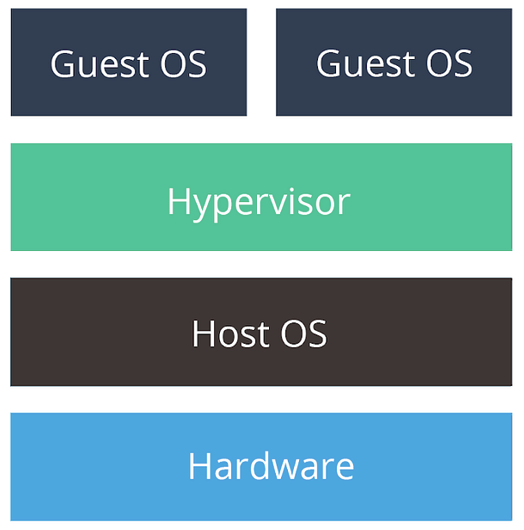
\includegraphics[width=0.7\linewidth]{images/Technologies/type_2_hypervisor.png}
	\caption{Type 2 (or hosted) hypervisor architecture \cite{HypervisorsArchitectures}.}
	\label{fig:type_2_hypervisor}
\end{figure}

Even though VirtalBox relies on the host OS for certain operations, which can lead to performance differences and potential resource conflicts, it was chosen over a type 1 hypervisor for its user-friendly virtualization solution.

The installation process involved creating a virtual disk, configuring memory and CPU allocation and selecting the Ubuntu 22.04 ISO file previously downloaded for installation \cite{UbuntuISOImage}. 
The virtual machine provided a native Linux platform for eBPF program development, compilation and testing.


\section{Virtual machine for Windows development}

Since the main focus is the analysis of eBPF state of art on Windows, the project also demanded the capability to develop eBPF programs specific to the Windows platform. 
For this purpose, the Hyper-V Console Manager, a native Windows feature, was used to create a separate Windows 11 virtual machine.

Hyper-V is a type 1 or bare-metal virtualization software, also known as a Virtual Machine Monitor (VMM), which runs directly on the physical hardware without the need for an underlying host operating system. 
The illustrative representation of the architecture just described is depicted in Figure \ref{fig:type_1_hypervisor}.
As the core software responsible for managing virtual machines and allocating hardware resources to each VM, Hyper-V ensures better security and resource utilization by isolating each VM from others and the host OS. 
With direct access to the physical hardware, it efficiently allocates resources, resulting in improved performance, isolation and scalability compared to type 2 hypervisors like VirtualBox.

\begin{figure}[h]
	\centering
	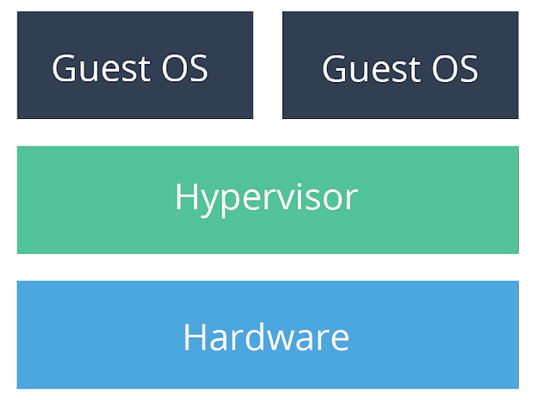
\includegraphics[width=0.7\linewidth]{images/Technologies/type_1_hypervisor.png}
	\caption{Type 1 (or bare metal) hypervisor architecture \cite{HypervisorsArchitectures}.}
	\label{fig:type_1_hypervisor}
\end{figure}

Even though hypervisors are favored for their robustness and scalability, enabling the efficient virtualization of large-scale applications and services, the choice of creating a virtual machine using the Hyper-V Console Manager was dictated by the setup instructions described on the \textit{ebpf-for-windows} GitHub repository \cite{VMSetup}.

We are going to talk about the eBPF installation on Windows later: for now, besides the fact that that he virtual machine was configured with adequate resources to support development tasks effectively, the only thing worth noting is that during the quick creation of the virtual machine the option of ``Windows 11 dev environment'' must be selected (the tutorial tells to choose the ``Windows 10 dev environment'', but Windows 11 works as well).  

The so created isolated Windows 11 development environment provided a controlled space for testing and optimizing eBPF programs on the Windows platform.

\section{Repository of the project}

GitHub is a platform and cloud-based service for software development and collaborative version control using Git, a distributed version control system that tracks changes in any set of computer files, allowing developers to store and manage their code, owned by the company GitHub Inc., whose logo is displayed in Figure \ref{fig:GitHub_logo}.
It provides the distributed version control of Git plus access control, bug tracking, software feature requests, task management, continuous integration and wikis for every project.
It is commonly used to host open source software development projects.

\begin{figure}[h]
	\centering
	
\includegraphics[width=0.7\linewidth]{images/Technologies/GitHub_logo.png}
	\caption{GitHub \textit{Invertocat} logo \cite{GitHubLogo}.}
	\label{fig:GitHub_logo}
\end{figure}

GitHub has been an invaluable platform for sharing the progress of my work with my co-advisors and facilitating collaboration during the entire development process. 
Its version control system allowed me to keep track of changes, maintain a detailed history of my project and collaborate consistently with my co-advisors, ensuring a smooth and efficient development workflow. 
By regularly pushing updates to the repository \cite{MasterThesisRepo}, my co-advisors were able to monitor the evolution of my work, review code changes, provide timely feedback and offer valuable suggestions for improvement.

Beyond the immediate scope of my thesis, the public visibility of the GitHub repository opens up the possibility of sharing my work with the broader community. 
By making the repository public, we hope that others can benefit from the knowledge and insights gained during the project, encouraging collaboration and contributions from future researchers and developers.

\todo{CITARE TEXSTUDIO E LATEX}

\chapter{The history of eBPF}

This chapter digs in the historical journey of extended Berkeley Packet Filter (eBPF), starting from the first ideas of packet filtering to its current state as a powerful and versatile technology. 
By exploring the foundations of packet filtering and the development of traditional BPF, we lay the groundwork for understanding the motivations behind eBPF's emergence. 
We will uncover how eBPF has revolutionized networking, observability and security in contemporary computing environments, from its initial applications in Unix-based systems to its widespread adoption in modern computing.

\section{The beginning of packet filtering}

The acronym BPF was first used in December 1992 in a document written by Steven McCanne and Van Jacobson while working at Lawrence Berkeley Laboratory (Berkeley, California, USA), titled \textit{The BSD Packet Filter: a New Architecture for User-level Packet Capture} \cite{BSDPacketFilter} and presented at the 1993 Winter USENIX conference in San Diego, California, USA (it is just an 11 pages document and it is worth giving it a read).
Fun fact, at the beginning of its story, the \textit{B} in BPF stood for Berkeley Software Distribution (BSD), a discontinued operating system based on the early version of Unix, which was developed and distributed by the Computer Systems Research Group at the University of California in Berkeley: in fact, at its beginning, BPF was running only on the FreeBSD operating system.

In this article they talk about the packet-capture techniques existing at the time and they describe the BSD packet filter (BPF) including its placement in the kernel and implementation as a virtual machine, defining it as ``a new kernel architecture for packet capture''.
The authors first start to describe the need to manage network traffic efficiently and how it was performed with the facilities implemented to those days.
Then, they present the plan behind BPF, showing its model and designing a virtual machine (perhaps, the most important thing) that would work as a filter with BPF, emphasizing on expandability, generality and performance.
They defined the design of the virtual machine by the following five statement:

\begin{itemize}
	\item ``It must be protocol independent. The kernel should not have to be modified 
		to add new protocol support.'';
	\item ``It must be general. The instruction set should be rich enough to handle unforeseen uses'';
	\item ``Packet data references should be minimized.'';
	\item ``Decoding an instruction should consist of a single C switch statement.'';
	\item ``The abstract machine registers should reside in physical registers.''.
\end{itemize}

In the end, they do some examples of packet filtering with BPF and with other technologies to compare their performances on the same hardware, showing how and why BPF performs substantially better than other approaches.

There are two last things that are worth noting in this paper.
First, when the paper was published, BPF was approximately two years old in which it had been tested and already found its way into multiple tools
This shows that the development of BPF was a gradual one, something that continues with the technologies that succeeded it.
Second, it mentions tcpdump as the program that uses BPF the most at the time of writing.
tcpdump is a data-network packet analyzer computer program that runs under a command line interface and allows the user to display TCP/IP and other packets being transmitted or received over a network to which the computer is attached.
Still to our days, it is one of the most widely used network debugging tools: this shows that tcpdump has used BPF technology for at least thirty years.
Funny enough, tcpdump is free software written in 1988 by a team of people including Van Jacobson and Steven McCanne who were, at the time, working in the Lawrence Berkeley Laboratory.

\section{The characteristics of BPF}

While the previous article was the first to cover BPF, it offers a broad view of the improvements this technology would bring to the world of network monitoring:

\begin{itemize}
	\item It outperformed other facilities of that time in their filtering mechanisms;
	\item It had a programmable pseudo-machine model that demonstrated to be general 
		and extensible;
	\item It was portable and ran on most BSD systems which, due to 
		their Unix-like basis, were a synonym of high quality networking back then;
	\item It could interact with various data-link layers.
\end{itemize}

Given these characteristics, it can be understood how BPF was ahead of its time: it was used to speed up packet filtering and analyze network traffic, since packets rates could be very high, even for the computers at the time when McCanne and Jacobson wrote their article. 
In fact, the original BPF was designed for capturing and filtering network packets that matched specific rules: to do so, a user-space process was allowed to supply a filter program that specifies which packets it wants to receive.
Then, the filter programs were interpreted by the Linux kernel and executed by the virtual machine.

The fact that BPF worked in a way similar to a virtual machine in the kernel was the most interesting part about this new technology because it was the thing that BPF did so differently that its predecessors: it used a well thought out memory model and then exposed it through an efficient virtual machine inside the kernel. 
Without requiring the overhead of copying packets between user space and kernel space, BPF filters could do traffic filtering in an efficient manner while still maintaining a boundary between the filter code and the kernel.

The features of this virtual machine are described in the document mentioned above: it was a 32-bit machine with fixed-length instructions, ``an accumulator, an index register, a scratch memory store, and an implicit program counter''.
Programs in that language could perform different types of operations, like fetching data from the packet, performing arithmetic operations on data from the packet and comparing the results against constants or against data in the packet or test bits in the results, accepting or rejecting the packet based on the results of those tests.

But how can traditional Unix-like BPF implementations be used in user-space, despite being written for kernel-space? 
This is accomplished using preprocessor conditions.
A preprocessor is a program that receives an input and produces an output that it will be used as an input for an other program.
This is a typical features of compilers, computer programs that translate computer code written in one programming language (the source language) into another language (the target language). 
This name is primarily used for programs that translate source code from a high-level programming language to a low-level programming language (e.g. assembly language, object code, or machine code) to create an executable program.
We brought the example of compilers because we are going to see later that the process of loading a BPF program inside the kernel requires, among many things, a compiler.

An other interesting feature about BPF was the fact that it provided a raw interface to various data-link layers, allowing it to work with different types of network interfaces and packet formats.
This feature made it a powerful tool for packet filtering and analysis across different network technologies, making possible to apply BPF in a wide range of networking scenarios
Sometimes, BPF is used specifically in reference to its filtering capabilities, rather than encompassing the entire interface. 
Across various systems, like Linux, other raw interfaces to the data link layer exist and they utilize BPF's filtering mechanisms for their own purposes. 

\section{Limitations of BPF}

The decision to run user-supplied programs within the kernel proved to be highly advantageous, but certain aspects of the original BPF design faced difficult challenges over time:

\begin{itemize}
	\item The virtual machine and its fixed-length instruction set architecture (ISA, 
		a part of the abstract model of a computer that defines how the CPU is controlled by the software) were outpaced as modern processors transitioned to 64-bit registers and introduced new instructions for multiprocessor systems, such as the atomic exchange-and-add instruction (XADD),compromising its ability to efficiently handle complex tasks on contemporary hardware;
	\item The initial focus on offering a limited number of Reduced Instruction Set
		Computer (RISC, a computer architecture designed to simplify the individual instructions given to the computer to accomplish tasks in order to achieve higher performances) instructions no longer aligned with the demands of contemporary processors because it did not provide a sufficient instruction set to handle advanced filtering and analysis task effectively;
	\item As new networking functionalities emerge, incorporating them into the 
		traditional BPF framework became challenging, because it lacked robust mechanisms for extensions and overloading of instructions, making very difficult its adaptability to ever-evolving network architectures;
	\item Since BPF was primarily designed for execution within the kernel space,
		its use in certain user-space scenarios and in other potential applications was limited due to its lack of versatility;
	\item As modern networks handle higher data rates and voluminous traffic,
		processing and filtering massive amounts of packets in real-time with BPF could cause performance bottlenecks, impacting overall system responsiveness, because it might not scale efficiently;
	\item BPF was missing built-in safety mechanisms, making it vulnerable to errors
		or malicious code which could lead to system crashes or security breaches;
	\item BPF was not designed to handle efficiently complex packet structures or
		protocols, limiting its ability in analyzing and filtering non-standard or highly intricate network traffic;
	\item As networking technologies continue to evolve rapidly, BPF's rigidity 
		may create challenges in adapting to emerging protocols, data formats and network architectures, potentially making it less suitable for future innovations.
\end{itemize} 

It is essential to consider these limitations when evaluating the appropriateness of  BPF for modern networking requirements. 
In fact, all of the problems about BPF described above can be referred to the fact that in the IT world things evolve really quickly and at its beginning BPF was not flexible and extensible to the innovations that would be introduced in the years to come.

Recognizing its historical significance and contributions, it is clear that BPF was not enough to keep up with the technological advancements that would be done in modern hardware.
To try to address many of the described limitations, in 2014 \textit{Extended BPF} (eBPF), a more versatile and future-ready technology for advanced networking and observability needs, was introduced by Alexei Starovoitov and Daniel Borkmann, creators and current maintainers of this project.

\section{Introduction to eBPF}

eBPF is a technology that can run sandboxed programs in a privileged context such as the operating system kernel.
Therefore, eBPF enables the safe and efficient extension of kernel capabilities without the need to modify kernel source code or load kernel modules.

Historically, the operating system has been an optimal platform for implementing the functionalities that eBPF was designed for (e.g. observability, security, and networking) because it benefits from the kernel's privileged ability to oversee and control the entire system.
However, evolving an operating system kernel is very challenging due to its central role and critical need for stability and security, resulting in traditionally lower innovation rates compared to functionalities implemented outside the operating system.
eBPF radically transforms this approach by enabling the execution of sandboxed programs within the operating system, empowering application developers to add extra capabilities at runtime. 
With the help of a Just-In-Time (JIT) compiler and a verification engine, the operating system also ensures a safe and efficient execution of the programs: in fact, compiling programs into native machine code that could be executed directly by the CPU, addressed the limitations of cBPF regarding the lack of performance and flexibility, improving the execution speed and versatility of eBPF programs compared to the cBPF filtering programs that were written in assembly-like instructions that 
represent the bytecode and they were interpreted by the kernel's cBPF interpreter that processes each instruction in the program sequentially for every packet.

eBPF has first appeared in the Linux kernel version 3.18 released in December 2014 after the extension of the inner BPF virtual machine and makes the original version, which has been retroactively renamed to \textit{classic} BPF (cBPF), mostly obsolete.
In Table \ref{table:cBPF_vs_eBPF} we can see the main differences that were brought with the introduction of eBPF.

\begin{table}[h]
	\centering
	\begin{tabular}{|| l | l | l ||} 
		\hline
		& Classic BPF & Extended BPF \\
		\hline
		\hline
		Word size & 32-bit & 64-bit \\
		\hline
		Registers & 2 & 10+1 \\
		\hline
		Storage & 16 slots & 512 byte stack + infinite map storage \\	
		\hline
		Events & packets & many event sources \\
		\hline
	\end{tabular}
	\caption{Comparison between cBPF and eBPF main features.}
	\label{table:cBPF_vs_eBPF}
\end{table}

Moving to 64-bit registers and an increasing the number of registers from two to ten (since modern architectures have far more than two registers), allowed parameters to be passed to functions in eBPF virtual machine registers just like on native hardware and virtually gave the virtual machine unlimited storage.
If you want to read the details about the differences between cBPF and eBPF you can check ``The Linux Kernel Archives'' document that talks about this topic \cite{cBPFvseBPF}.

While these changes were introduced in eBPF due to the progresses made in computer hardware, there have also been several revolutions regarding the technology itself:

\begin{itemize}
	\item The most important one is the fact that an eBPF program, instead of only
		being attached to packets, it can now be attached to many different event sources and run many programs within the kernel, making this technology very powerful and allowing it to start being used in a wide variety of applications, including networking and tracing;
	\item At the lowest level, beyond the use of ten 64-bit registers, eBPF
		introduced different jump semantics, a new \textit{BPF\_CALL} instruction to call in-kernel functions cheaply and corresponding register passing convention, new instructions and a different encoding for these instructions;
	\item The ease of mapping eBPF to native instructions made it suitable for
		JIT compilation, which was supported by many architectures, bringing an improvement in the performance (``The original patch that added support for eBPF in the 3.15 kernel showed that eBPF was up to four times faster on x86-64 than the old cBPF implementation for some network filter microbenchmarks, and most were 1.5 times faster'' \cite{eBPFThroughIntroduction});
	\item eBPF was made more flexible and as the Linux kernel evolved in versions
		after 3.18, new functionalities (that we will discuss later) were subsequently added, such as the use of loops.
	\item More efficient global data stores, which eBPF calls ``maps'', were 
		introduced, allowing the state of a process to persist between events and thus be aggregated for uses including statistics and context aware behavior (we will discuss about them in the next chapter).
\end{itemize}

The described changes made eBPF appear to the world as a revolution.
Originally, eBPF was only used internally by the kernel and loaded cBPF bytecode was transparently translated into an eBPF representation in the kernel before program execution.
Finally, in 2014 the eBPF virtual machine was exposed directly to user space and nowadays the Linux kernel runs eBPF only.
Moreover, in 2021, due to its success in Linux and its simple virtual machine on which eBPF runs, the eBPF runtime has been ported to other operating systems such as Windows.
cBPF, instead, passed to history as being the packet filter language used by \textit{tcpdump}.

\section{What is eBPF?}

Even though the name Extended Berkeley Packet Filter hints at a packet filtering specific purpose, the instruction set was made generic and flexible enough that nowadays there are many use cases for eBPF apart from networking. 
In fact, eBPF is a highly flexible and efficient virtual machine-like construct with origins in the Linux kernel allowing to execute bytecode at various hook points in a safe manner: it processes a virtual instruction set and provides a safe way to extend kernel functionalities.
To make a comparison with a famous programming language we can say that eBPF does to the kernel what JavaScript does to websites: it allows the creation of all sort of applications.
It is used in a number of Linux kernel subsystems, most prominently networking, tracing and security (e.g. sandboxing).

The mind-blowing feature about eBPF is the fact that, at its core, it allows a user (in some cases privileged) to inject near general-purpose code in the kernel. 
Such code will then be executed at some point in time, usually after certain events of interest happen in the kernel. 
In theory, this sounds really similar to Loadable Kernel Modules (LKM), the traditional way with which users could extend the features of the kernel.
In fact, LKM consist of a compiled general purpose C code loaded at run time inside the kernel and the code of a kernel module usually hooks into various kernel subsystems so that it gets automatically called upon the occurrence of certain events.
This has been useful for developers who want to implement support for new hardware devices or tracing functions, for example.
Even though both approaches want to extend the capabilities of the kernel at runtime, the big difference between them is the fact that, unlike LKM, eBPF will only run code that has been evaluated completely safe to run.
This means that it will never lead to a kernel crash or kernel instability, which is something currently difficult to achieve with other technologies without giving up some serious flexibility. 
We could say that eBPF does the same job as LKM, but it does not require to change kernel source code or load kernel modules and does it in a safe and efficient manner.

How could this safety be achieved? It is provided through an in-kernel verifier which performs static code analysis and rejects programs which crash, hang or otherwise interfere with the kernel negatively (e.g. programs without strong exit guarantees like loops without exiting conditions, programs dereferencing pointers without safety-checks, ...).
Programs that pass the verifier are loaded in the kernel where they will JIT compiled for native execution performance.
Once again, the compiled eBPF program is verified before running to prevent denial-of-service attacks.
Due to the fact that the execution model is event-driven, programs can be attached to various hook points in the operating system kernel and are run upon triggering of a specific event.

\section{eBPF in modern architecture}

\subsection{Name and logo}

Nowadays, BPF is a technology name and no longer just an acronym because its use case outgrew networking, even though it evolved from BPF as an extended version.
Due to the fact that the acronym does no longer make a lot of sense, eBPF is now considered a standalone term that does not stand for anything.
Some people still call it eBPF to really make the point that it's new: however kernel engineers tend to stick to BPF, meaning a generic internal execution environment for running programs in the kernel.
Moreover, BFP adn eBPF are generally used interchangeably in documentation and various tools.
Consistently with the research aim of this thesis, we are going to distinguish eBPF from cBPF to make more clear what we are referring to, even if from this point on we are going to talk exclusively about eBPF.

eBPF was also provided with an official logo: at the first eBPF Summit there was a vote taken and they decided to use the bee, named ``eBee''.
So, Vadim Shchekoldin created the eBPF logo, which we can see in Figure \ref{fig:eBPF_logo}.

\begin{figure}[h]
	\centering
	
\includegraphics[width=0.7\linewidth]{images/History/eBPF_logo.png}
	\caption{eBPF logo.}
	\label{fig:eBPF_logo}
\end{figure}

\subsection{eBPF Foundation}

Since its introduction in the infrastructure software world, the number of eBPF-based projects has exploded in recent years and more and more companies announced their intent to start adopting this technology.
As such, there was the need to collaborate between projects to ensure that the core of eBPF would be well maintained and equipped with a clear path and vision for the bright future ahead of eBPF.

To respond to this demanding need, in August 2021, some companies, including Meta, Google, Microsoft, Isovalent and Netflix, founded the ``eBPF Foundation'', establishing an \textit{eBPF steering committee} (BSC) to take care of the technical direction and vision of eBPF.
As one might expect, among the few members of the committee, there are Alexei Starovoitov and Daniel Borkmann.
The logo of this institution can be seen in Figure \ref{fig:eBPF_foundation_logo}

\begin{figure}[h]
	\centering
	
\includegraphics[width=0.7\linewidth]{images/History/lf-stacked-color.png}
	\caption{eBPF Foundation logo.}
	\label{fig:eBPF_foundation_logo}
\end{figure}

The purposes of this foundation are various and numerous:

\begin{itemize}
	\item Expand the contributions being made to extend the powerful capabilities of
		eBPF and grow beyond Linux (as we already mentioned before, eBPF is now also available on Windows);
	\item Raise funds in support of various open source, open data and/or open
		standards projects relating to eBPF technologies to further drive the growth and adoption of the eBPF ecosystem;
	\item Defining the minimal requirements of eBPF runtimes and maintain eBPF
		technical project lifecycle procedures to ensure a smooth and efficient progress of eBPF initiatives;
	\item Create a strong community that would collaborate among projects, attend
		technical workshops and conferences to discuss ongoing research, development efforts and use cases around eBPF.
\end{itemize} 

Basically, the foundation wants to get as many people as possible to adopt eBPF and involve them into the project.
To do so, they also created a place where everybody can learn and collaborate to the topic of eBPF which is called \textit{eBPF.io} \cite{eBPFioWebsite}.
Throughout the years eBPF has been surrounded with an open community and everybody can participate and share: eBPF.io is a website where anyone can learn something about eBPF, from reading a first introduction to listen to some community talks, and become a contributor to major eBPF projects.

\subsection{Use cases of eBPF}

We understood that eBPF programs are verified within the kernel to avoid various threats: therefore eBPF programs pose less risk compared to an arbitrary loadable LKM and they also impose less overhead for many observation tasks compared to related tools.
For this reasons, throughout the years, many more companies have joined this project and stated using eBPF.
Nowadays, eBPF has been adopted by a number of large-scale production users, like Google, Meta, Netflix, Apple, Android, Microsoft,... mostly for network observability, security enforcement and layer 4 (in the ISO/OSI model) load balancing.

However, due to the fact that eBPF is very versatile, performing and programmable, people have found innovative solutions in various areas:

\begin{itemize}
	\item Thanks to the networking and security revolution, eBPF allows administrators
		to create custom filters and access controls at the kernel level, offering powerful packet filtering and firewall capabilities while minimizing performance overhead (firewalls, intrusion detection systems and DDoS protection.);
	\item Given eBPF's real-time observability capabilities, achieved by attaching
		programs to kernel hooks, enable developers to gain deep insights into system calls, network activity and resource utilization, empowering efficient monitoring with low-latency and non-intrusive measurements in the dynamic environment of many systems and applications;
	\item In containerized environments, eBPF emerges as a game-changer, allowing
		administrators to efficiently control and optimize network traffic between containers, improving isolation, security and performance while, thanks to its programmability, consistently aligning with the dynamic nature of container orchestration platforms, like Kubernetes;
	\item In the middle of the evolving cloud landscape, eBPF assumes a central role,
		enabling efficient load balancing, traffic shaping and service discovery within the cloud infrastructure, ensuring optimal resource utilization and networking agility;
	\item Developers are enabled to look into application behavior and system
		performance through event capture and analysis at the kernel level using tracing tools that serve as instrumental support for diagnosing	performance issues and debugging complex systems;
	\item eBPF is also used for real-time protection against malicious network
		activities due to the fact that it allows Intrusion Prevention Systems (IPS) to quickly inspect and filter packets, enabling rapid threat detection and prevention, while applying custom security policies and filtering rules;
	\item To reduce latency and increase efficiency for critical networking functions,
		eBPF uses custom in-kernel processing, efficiently offloading specific tasks to eBPF programs.
\end{itemize}

To summarize what we have seen until now, eBPF has only been in the Linux kernel since 2014, but has already worked its way into a number of different uses in the kernel for efficient event processing (socket filtering, capturing information, analyzing performances, attaching programs to hook points or probes,...). 
However, the modern use of eBPF continues to expand, as developers and organizations explore its capabilities and integrate it into various innovative applications. 
With its ever-growing ecosystem of tools, libraries and frameworks, eBPF is at the vanguard of driving efficiency, security and observability in contemporary computing environments.

\section{The portability of eBPF}

During our discussion, we mentioned the fact that eBPF tools surround functionalities in both kernel and user space, which aim at providing stable interfaces, such as kernel and user space tracepoints. 
However, it's essential to note that eBPF tools can also refer to functionality like functions or field names in the kernel that may lack stability. 
For this reason, eBPF programs may not be portable across different kernels.

In fact, the main priority of the eBPF community since its creation was to make the development od eBPF application as simple as possible, making it a similar experience to developing any application in user-space.
Even though there were many usability improvements during the years, the aspect of portability has always been forsaken (mostly for technical reasons).

``BPF portability is the ability to write a BPF program that will successfully compile, pass kernel verification, and will work correctly across different kernel versions without the need to recompile it for each particular kernel'', says Andrii Nakryiko, a kernel engineer at Meta and member of the BSC, in a post \cite{ANCOREPost} published on his blog \cite{ANBlog}.
For example, one of the natural challenges for tools that use kernel data structures (like eBPF) is that the offsets for fields can vary based on kernel version and configuration.

\subsection{The problem of portability}

So far we understood that the power of eBPF is the fact that a piece of user-provided code (the program) is injected straight into a kernel and, after the phases of verification and loading, executes in kernel context, operating inside kernel memory space with access to all the internal kernel state available to it. 
However, at the beginning of eBPF this powerful capability also created some portability problems: eBPF programs do not control memory layout of a surrounding kernel environment. 
This means that they have to work with what they get from independently developed, compiled and deployed kernels.

Moreover, new kernel versions are continuously released (as of September 2023 the Linux kernel is at version 6.5, far from the 3.18 of December 2014): so, kernel types and data structures are in constant flux.
The problem is that kernel version may differ under various architectural aspects: struct fields are shuffled around inside a struct or even moved into a new inner struct, fields can be renamed or removed, their types changed, either into some compatible ones or completely different ones, structs and other types can get renamed or just plain removed.

Even if not all eBPF programs need to look into internal kernel data structures and eBPF machinery inside kernel provides a limited set of stable interfaces that eBPF programs can rely on to be stable between kernels (in reality, underlying structures and mechanisms do change, but these eBPF-provided stable interfaces abstract such details from user programs), things change all the time between kernel releases and yet BPF application developers are expected to address this problem in some way. 

Even if not all eBPF programs require direct access to kernel data structures and the eBPF framework offers a limited set of stable interfaces that abstract changes between kernel versions (underlying structures and mechanism do change), things mutate all the time between kernel releases and yet BPF application developers are expected to address this problem in some way. 

\subsection{The temporary solution: BCC}

The first thing that people started using for addressing this problem is \textit{BPF Compiler Collection} (BCC) \cite{BCCGitHub}, a toolkit for creating kernel programs suited for different tasks, such as network traffic and performance analysis.
To make sure that the running kernel's memory layout is the same as the one expected by the eBPF program, when the application is executed by the host, BCC calls its embedded Clang/LLVM, puts the headers into the kernel and does compilation on the fly.
Additionally, you can define and rename any optional stuff not available on the kernel configuration that you are using and the Clang will adapt your eBPF program code to the specific kernel.

While this workflows work, it has some problems.
Firstly, the Clang/LLVM combo is a big library and resource heavy: this means that you have to install big binaries when you distribute your application and the process of compilation can require a lot of time.
Secondly, you have to hope that the system on which you are going to install your application has the kernel headers present, because BCC-based application do not work on kernels that have been custom built.
Lastly, working in an agile method is quite difficult because you will get compilation errors only at runtime and you have to recompile and restart your application every time.

Although BCC is a great tool for experimenting small tools, when we look at some example of widely deployed, complex and real-world eBPF application we have to think of an other solution.

\subsection{The solution: BPF CO-RE}

\textit{BPF Compile Once - Run Everywhere} (BPF CO-RE) is a feature in the eBPF ecosystem that aims to solve the problem of portability of eBPF programs across different versions and architectures of the Linux kernel which was presented at the ``Linux Storage, Filesystem and Memory Management (LSF/MM) Summit for 2019''.

BPF CO-RE allows to easily write portable eBPF programs: to do so, it requires the integration and the cooperation of different components:

\begin{itemize}
	\item \textit{BPF Type Format} (BTF), a compact, but expressive enough format to
		describe the information of C programs, that is used to enhance the verifier's capabilities;
	\item A support for the compiler, as Clang  had to be extended with built-ins that
		allow the capture of field offset, existence and size, type size and relocation and enum values and existence;
	\item A loader, named \textit{libbpf} \cite{libbpfGitHub}, that takes the BPF
		object file (the program after its compilation) and triggers the phases of loading and verification;
	\item The kernel, which does not need many changes to support BPF CO-RE.
\end{itemize}

With BPF CO-RE, eBPF programs are compiled into a more compact, intermediate representation that can be loaded and executed by various kernel versions.
This reduces the need to recompile programs for different kernel versions, making eBPF programs more portable and efficient. 

To enable BPF CO-RE and let eBPF loader to adjust an eBPF program to a particular kernel running on target host, the new built-ins for Clang release \textit{BTF relocations} which capture a high-level description of what pieces of information the eBPF program code want to read.
If you want to access a certain field in a struct inside the kernel and this field has been moved to a different offset inside the same struct or even to a different struct, the developer can find that field by just its name and type information.

Once we have the object file of the compiled eBPF program, the Clang relocations and the BTF information provided by the running kernel of the host, the loader makes sure that the logic of that program is correctly functioning for the specific kernel by matching these information.

The result is that it looks like the program was compiled specifically for the kernel of that machine, but this happened without distributing Clang with your application and performing compilation in runtime on target host.
In fact, thanks to a good separation of concerns, after the loader has processed the eBPF program, from the kernel perspective you see a valid eBPF program code (and everything is done without worrying about the kernel version).

\subsection{BPF CO-RE as today}

BPF CO-RE is now a mature technology used across a wide variety of projects: it is used for the development of many eBPF-based applications, due to its capability to handle, in a single compiled-once eBPF, application both simple cases of changing field offsets and much more advanced cases of kernel data structures being removed, renamed or completely changed.

We understood how BPF CO-RE helped the developers to solve the portability issues of eBPF.
We do not have to forget that it also provides a good usability and familiar workflow of compiling C code into binary and distributing lightweight binaries around. 
This eliminated the need to install a heavy-weight compiler library together with your application and the cost of precious runtime resources for runtime compilation. 
Furthermore, there is no more need to catch sneaky compilation errors at runtime.

There are other complex things that BPF CO-RE makes easier for the user for dealing with different kernel versions and configuration differences: the curious ones can read more about this topic on Nakryiko's post \cite{ANCOREPost}.

\section{Future and potential of eBPF}

In the previous paragraph we showed how the problem of portability was resolved.
However, certain older kernels might not incorporate the required functionality and some kernels may lack the necessary configuration to support eBPF. 
As a result, it becomes evident that eBPF cannot be universally considered portable or available.
In fact, even if eBPF is now supported on multiple platforms, as the beginning of 2023 there is no standard specification to formally define its components. 

Nevertheless, the world of eBPF evolves quickly and distributions appear to regularly support eBPF and provide a package of eBPF tools for easy installation. 
Furthermore, there is currently some work in progress to define and publish a standard for the instruction set, under the auspices of the eBPF Foundation.

So, for now, if you are running a recent version of the kernel and you can invoke eBPF as a privileged user, you should have eBPF functionality available.
But if some eBPF tools do not work with your kernel, do not get disappointed: there are many people that are joining forces to make eBPF programs more portable.

Despite the need to standardize the technology and integrate it into as many platforms as possible, making it more accessible to developers and organizations worldwide, the future of eBPF is bright, due to its potential to twist the world of modern computing.
This innovative technology is ready to unlock new frontiers and revolutionize various domains thanks to some key aspects:

\begin{itemize}
	\item As network requirements keep evolving, with the help of eBPF's 
		programmability, administrators have to implement newer custom network protocols, load balancing algorithms and traffic shaping mechanisms;
	\item As cloud adoption continues to rise, eBPF's indispensability in the
		cloud-native ecosystem will grow further, offering fine-grained control over container networking for optimal isolation, advanced security and efficient resource utilization, making agility and scalability essential for modern cloud infrastructure;
	\item The future of debugging and optimization for complex and distributed systems
		belongs to eBPF's real-time observability and tracing capabilities which allow developers to exploit its potential for capturing, analyzing and visualizing diverse system events with the purpose of providing unparalleled insights into application behavior, performance bottlenecks and resource utilization;
	\item As cyber threats become increasingly sophisticated, eBPF will persist in
		strengthening security measures, expanding its role in intrusion detection systems and security applications, providing real-time packet inspection, protocol analysis and advanced filtering capabilities;
	\item In a world where Artificial Intelligence and machine learning are
		increasingly in the spotlight, eBPF's programmability prepares to integrate them within the kernel, promoting a powerful synergy that drives intelligent decision-making, automated resource management and dynamic adaptation to satisfy shifting workloads and network conditions;
	\item With the help of the thriving eBPF community, new tools, libraries and
		frameworks are developed rapidly, pushing the boundaries of eBPF's potential and encouraging the creation of innovative solutions.
	\item As the world of Internet of Things and edge computing expands, eBPF's
		lightweight and efficient nature makes it an ideal match for devices with limited resources, finding applications in intelligent edge gateways for data filtering, analysis and real-time decision-making;
\end{itemize}

It’s highly likely that the trend of using eBPF for safe and efficient event handling will continue.
Thanks to its restrictive and simple implementation, eBPF offers a highly portable and performant way to process events. 
More than that, however, eBPF makes a change in how problems are solved: instead of using objects and stateful code, it exploits just functions and efficient data structures to store state. 
By doing so, the possibilities of a program’s design are reduced, but allows eBPF to be used with nearly any method of program design (synchronously, asynchronously, in parallel, distributed, ... depending on the coordination needs with the data store).

In conclusion, the future and potential of eBPF are full with possibilities. 
As it evolves, eBPF is set to reshape networking, observability and security paradigms, enabling developers to build efficient, secure and adaptable systems in the always evolving world of computing. 
With its impact and large adoption, eBPF is ready to become a landmark of next-generation software-defined infrastructures and beyond.

\todo{https://www.ferrisellis.com/tags/ebpf/ -> PART 1 -> KERNEL-SPACE VM ?}
\todo{NEW COMMANDS}
\chapter{The eBPF subsystem}

From what we have learned from the previous chapter we can try to give a definition to eBPF: it is a ``verified-to-be-safe, fast to switch-to mechanism, for running code in Linux kernel space to react to events such as function calls, function returns, and trace points in kernel or user space'' \cite{eBPFLinuxJournal}.
In a few words, eBPF is very powerful because it is fast and it is safe. 

Given also eBPF's efficiency and flexibility, Brendan Gregg, an internationally famous expert in computing performance,  famously coined eBPF as ``superpowers for Linux''.
Linus Torvalds, the author of the first version of the Linux kernel, expressed that ``BPF has actually been really useful, and the real power of it is how it allows people to do specialized code that isn't enabled until asked for''.
Once again, we mention the fact that due to its success in Linux, the eBPF runtime has been ported to other operating systems such as Windows.

Like all superheroes are shocked when they first come across their superpowers, eBPF too can seem overwhelming at first glance.
To fully appreciate it, the goal of this chapter is to explain everything you need to know about eBPF.

\section{Writing an eBPF program}

In the previous chapter we understood the fact that, to achieve safety guarantee, eBPF is essentially implemented as a process virtual machine in the kernel which runs safe programs on behalf of the user.
eBPF exposes to the user a virtual processor, with a custom set of RISC-like instructions and also provides a set of virtual CPU registers and a stack memory area.
Thanks to this features, developers can write programs in eBPF bytecode (the form in which the Linux kernel expects eBPF programs) and pass them to the virtual machine to be evaluated.

While it is of course possible to write bytecode directly, developers do not have to create eBPF bytecode from scratch when writing a new program.
It has been implemented an eBPF back-end for Low-Level Virtual Machine (LLVM, ``a collection of modular and reusable compiler and toolchain technologies'' \cite{LLVMWebsite}): as a result Clang, the LLVM front-end compiler for C-derived programming languages, can be used to compile a subset of standard C code in an eBPF object file.
While the C to eBPF translation must be done in a very cautious way, it massively expands the use cases of eBPF due to the fact that it makes relatively easy to write new eBPF code in a familiar programming language such as C.

At this point it is important to mention that in a lot of scenarios, eBPF is used indirectly via projects like Cilium, bcc, bpftrace and many more. 
The peculiarity of these projects is the fact that they provide an abstraction on top of eBPF and do not require writing programs directly: instead, they offer the ability to specify intent-based definitions which are then implemented with eBPF.
If no higher-level abstraction exists, programs need to be written directly. 
We are going to look at some of this projects in the next chapter of this paper.

In the following we are going to look at the  components mentioned above and how they work in practice, including how the program safety verification is done.

\section{Architecture}

We understood that the architecture of eBPF (extended Berkeley Packet Filter) is characterized by its ability to provide programmability within the kernel, offering a powerful framework for safe and efficient extension of kernel functionality. 
At its core, eBPF operates as an in-kernel virtual machine, running sandboxed programs that are designed to enhance kernel behavior without requiring changes to the kernel source code or loading kernel modules.

When we talk about an eBPF program, we have to consider a big infrastructure of things that make this technology interesting:

\begin{itemize}
	\item The instruction set, which defines the main characteristics of eBPF;
	\item Maps, efficient key/value data structures;
	\item Helper functions, to exploit kernel functionalities;
	\item Tail calls, for calling into other eBPF programs;
	\item Hook points, which are points of execution in the kernel to which an eBPF 
		program	is attached;
	\item A verifier, a program used to determine the safety of a program;
	\item A compiler, used to compile the program in an object file that can be loaded
		in the kernel; 
	\item The kernel subsystem that uses eBPF.
\end{itemize}

When an eBPF program passes the verification process, it is then compiled, loaded in the kernel and attached to a hook point.
When the associated event or condition occurs in the kernel, the attached eBPF program is triggered to execute and it receives some input data coming from the kernel (e.g. the system call arguments passed by the user space process invoking the system call to the kernel, if the program is attached to a system call execution via a system call tracepoint): the program can then manipulate the input data tu perform various operations, such as filtering a packet (for networking use), compute a set of metric (typically for tracing, where the programs are attached to a very busy execution point in the kernel) or interact with the kernel, as defined by the program's logic.

The following paragraphs provide further details on individual aspects of the eBPF architecture.

\section{The instruction set}

In order to guarantee good performance on the kernel side, the RISC instruction set of an eBPF program is simple enough that it can be relatively easily translated into native machine code via a JIT step embedded inside the kernel. 
This means that right after the verification of the safety of the program, the runtime will not actually suffer the performance overhead of having to execute the eBPF bytecode via the virtual machine. 
It will just execute straight native machine code, significantly improving the performance.

Moreover, the general purpose RISC instruction set was designed for writing eBPF program in a subset of C which can be compiled into BPF instructions through a compiler back end (e.g. LLVM), so that the kernel can later on map them through an in-kernel JIT compiler into native opcodes for optimal execution performance inside the kernel.

There are several advantages for pushing these instruction into the kernel:

\begin{itemize}
	\item The kernel is made programmable without having to cross the boundaries
		between kernel-space and user-space;
	\item Programs can be heavily optimized for performance by compiling out features
		that are not required for the use cases the program solves;
	\item eBPF provides a stable Application Binary Interface (ABI, the machine
		language interface between the operative system and its applications) towards user space and does not require any third party kernel modules because it is a core part of the Linux kernel that is shipped everywhere, making eBPF programs portable across different architectures;
	\item eBPF programs work with the kernel, making use of existing kernel
		infrastructure (e.g. drivers, netdevices, sockets, etc.) and tooling (e.g. iproute2) as well as the safety guarantees which the kernel provides.
\end{itemize}

\section{Hook points}

eBPF programs are event-driven by design and are run when the kernel or an application triggers a certain \textit{hook point}. 
When the designated code path is traversed, any eBPF program attached to that point is executed.
In the kernel there are some pre-defined hooks, including system calls, function entry/exit, kernel tracepoints, network events and several others.
It is also possible to create custom hook points to attach eBPF programs almost anywhere in kernel or user applications by creating a kernel probe (kprobe) or user probe (uprobe).

Given its origin, eBPF works really well writing network programs and it's possible to write programs that attach to network sockets, enabling the user to do many different operations such as traffic filtering, classification and network classifier actions.
Even the modification of established network socket configurations can be achieved through eBPF programs.
A notable use case is the eXpress Data Path (XDP) project \cite{XDPWebsite}, which leverages eBPF to carry out high-performance packet processing by executing eBPF programs at the network stack's lowest level, immediately following packet reception.

In addition to network-oriented applications, we already discussed that eBPF has many other purposes: it can filter and restricting system calls, debug the kernel and carry out performance analysis.
To do so, programs can be attached to tracepoints, kprobes and perf (a tool to analyze performance in the Linux kernel) events.
Because eBPF programs can access kernel data structures, developers can write and test new debugging code without having to recompile the kernel (the implications are obvious for engineers whose work is to debug issues on live and running systems).

When the desired hook has been identified, the eBPF program can be loaded into the Linux kernel for verification and further use using the \textit{bpf} system call. 
This is typically done using one of the available eBPF libraries. 

\section{Compiling and loading an eBPF program}

Once we have decided where we want to attach our eBPF program (based on the operation that we want to do), the eBPF framework will start executing this program only after verifying that they are safe from an execution point of view. 

An eBPF program has to go through a series of steps before being executed inside the kernel.

\subsection{Compilation}

We already said that an eBPF program is written in a high-level programming language, such as C.
The first thing that happens to a program is its compilation using Clang with its eBPF backend LLVM: this process generates eBPF bytecode which resides in an Executable and Linkable Format (ELF, a standard file format for executables, object code, shared libraries, and core dumps.) file.

As this file is loaded into the Linux kernel, it passes through two steps before being attached to the requested hook: verification and JIT compilation.

\subsection{Verification}

There are security and stability risks with allowing user-space code to run inside the kernel. 
So, a number of checks are performed on every eBPF program before it is loaded. 
The generated eBPF bytecode undergoes verification by a safety tool, the eBPF \textit{verifier}, within the kernel to ensure that the eBPF program is safe to run.
It is not a security tool inspecting what the programs are doing.
The verifier checks the bytecode for safety, ensuring that it satisfies all the constraints and security rules to prevent potential security vulnerabilities.
The safety of the eBPF program is determined in two steps.

The first test ensures that the eBPF program terminates and does not contain any loops that could cause the kernel to lock up. 
To do so, the verifier does DAG check to disallow loops and a depth-first search of the program's control flow graph (CFG). 
Any program that contains unreachable instructions will fail to load, as they are strictly prohibited (though classic BPF checker allows them).
Furthermore, there must not be infinite loops: programs are accepted only if the verifier can ensure that loops contain an exit condition which is guaranteed to become true.

The second part requires the verifier to run all the instructions of the eBPF program one at the time: from the first instruction, the verifier descends all possible paths, simulating the execution of all instructions and observing the state change of registers and stack.
Then, the virtual machine state is checked before and after the execution of every instruction to ensure that register and stack state are valid. 
This step is done to check two major things: 

\begin{itemize}
	\item If programs are trying to access invalid memory or out-of-range data
		(outside the 512 byte of stack designated to each program), due to	the presence of out of bounds jumps, and use uninitialized variables because they should not have the ability to overwrite critical kernel memory or execute arbitrary code;
	\item If programs have a finite complexity (the verifier must be capable of
		completing its analysis of all possible execution paths within the limits of the configured upper complexity limit).
\end{itemize}

Although this second operation seems expensive in computation terms, the verifier is smart enough to know when the current state of the program is a subset of one it's already checked. 
Since all previous paths must be valid (otherwise the program would already have failed to load), the current path must also be valid. 
This allows the verifier to perform a sort of ``pruning'' to some branches and skip their simulation.

Another thing that is not generally allowed by the eBPF verifier is pointer arithmetic because it works under a ``secure mode'' which enables only privileged processes to load eBPF programs.
The idea is to make sure that kernel addresses do not leak to unprivileged users and that pointers cannot be written to memory. 
Unless unprivileged eBPF is enabled (and secure mode is not enabled), then pointer arithmetic is allowed but only after additional checks are performed (e.g. all pointer accesses are checked for type, alignment and bounds violations).

In general, untrusted programs cannot load eBPF programs: all processes that want to load eBPF programs in the kernel must be running in privileged mode.
However, you can enable ``unprivileged eBPF'' which allows unprivileged processes to load some eBPF programs subject to a reduced functionality set and with limited access to the kernel.

Lastly, the verifier uses the eBPF program type (covered later) to restrict which kernel functions can be called from eBPF programs and which data structures can be accessed. 
In fact, an eBPF program cannot randomly modify data structures in the kernel and arbitrary access kernel memory directly.
To guarantee consistent data access, an eBPF program running is allowed to modify the data of certain data structures inside the kernel only if the modification can be guaranteed to be safe and it can access the data outside of the context of the program via only eBPF helpers (which we will discuss later).

\subsection{Hardening}

Once the verifier has successfully completed his job, the eBPF program undergoes an hardening process according to whether the program is loaded from privileged or unprivileged process.

Hardening refers to the process of enhancing the security and safety of eBPF programs to prevent potential vulnerabilities and ensure their reliable and controlled execution within the kernel. 
This is particularly important because, as we already know, eBPF programs have the capability to run within the kernel's context, which requires robust measures to mitigate risks.

This step includes two main operations:

\begin{itemize}
	\item The kernel memory holding an eBPF program is protected and made read-only
		and any attempt to modify the eBPF program (through a kernel bug or malicious manipulation) will crush the kernel instead of allowing it to continue executing the corrupted/manipulated program;
	\item All constants in the code are blinded to prevent attackers from injecting
		executable code as constants which, in the presence of another kernel bug, could allow an attacker to jump into the memory section of the eBPF program to execute code (JIT spraying attacks, similar to JavaScript injection);
\end{itemize}

By following these practices, developers can minimize security risks and ensure that eBPF programs operate safely and reliably within the kernel's context, ensuring that only safe and well-behaved programs are allowed to run.
This process of hardening helps prevent potential security vulnerabilities and ensures the reliable and secure operation of eBPF programs.

\subsection{JIT compilation}

Once the bytecode has been verified and hardened, the eBPF JIT compiler is executed. 
It translates the verified eBPF bytecode into native machine code that corresponds to the target CPU architecture which can be directly executed by the processor. 
This native code is generated on-the-fly and is specific to the underlying hardware, ensuring optimal execution of eBPF programs by eliminating the overhead of interpreting bytecode.
The JIT compilation step makes eBPF programs run as efficiently as natively compiled kernel code or as code loaded as a kernel module.

In fact, JIT compilers speed up execution of the eBPF program significantly since they reduce the per instruction cost compared to the interpreter used in cBPF. 
Most of the times, instructions can be mapped one-to-one with native instructions of the underlying architecture. 
This also reduces the resulting executable image size of the program and is therefore more instruction cache friendly to the CPU.
Moreover, during JIT compilation, the compiler can apply various optimization techniques to enhance the efficiency of the generated machine code, which aim to reduce redundant operations, improve memory access patterns and optimize CPU registers allocation.

\subsection{Loading and execution}

The resulting native machine code is then loaded into the kernel's memory space: this is done in Linux using the \textit{bpf()} system call (see the next paragraph).
When the predefined event or hook associated to the eBPF program is triggered (e.g., a network packet arrival or a system call), its native machine code generated by the JIT compiler is executed directly by the CPU. 
This execution is significantly faster than interpreting bytecode, leading to improved performance.

As eBPF serves diverse purposes across various kernel subsystems, each eBPF program type has a distinct procedure for attaching to its relevant system. 
Once the program is attached, it becomes operational, engaging in activities such as filtering, analysis or data capture, according to its intended function. 
Subsequently, user-space programs can manage active eBPF programs, involving actions like reading states from eBPF maps and, if designed accordingly, modifying the eBPF map to influence program behavior.

Furthermore, while the program is running, the JIT compilation process allows for dynamic adaptation of the eBPF program's behavior based on the runtime environment: if changes occur in the system or the program's requirements, the eBPF JIT compiler can recompile the bytecode into a different native machine code to ensure optimal performance.

\section{The bpf() system call}

% https://www.ferrisellis.com/content/ebpf_syscall_and_maps/

The creation of the eBPF program as byte code and attaching the loaded program to a system in the kernel are two steps in the process of using an eBPF program that vary by use case.
However, the step in between these two, that is loading the program into the kernel and creating necessary eBPF-maps, is the core of eBPF and it is what all eBPF applications have in common.
In Linux, this step is done by the \textit{bpf()} system call, which was introduced in the Linux kernel version 3.18, released on the 7th of December 2014, along with the underlying machinery in the kernel: it is an interface provided by the Linux kernel that allows user programs to interact with and utilize eBPF functionality. 
It serves as a bridge between user space and the kernel, acting as a gateway for user applications to utilize the power of eBPF within the kernel.
This system call allows for the byte code to be loaded along with a declaration of the the type of eBPF program that’s being loaded and provides many more key functionalities, such as program execution, maps initialization for data exchange, helper function invocation and error handling.

Below we can see the necessary syntax of this system call:

\begin{lstlisting}[language=C]
	#include <linux/bpf.h>
	int bpf(int cmd, union bpf_attr *attr, unsigned int size);
\end{lstlisting}

The first line is a must when we want to exploit eBPF functionality: the \textit{linux/bpf.h} header file in the Linux kernel contains a collection of macro definitions, function prototypes and data structures related to the eBPF subsystem and programs. 
This header file provides the necessary interfaces and definitions for user space programs to interact with the eBPF subsystem in the kernel: it includes various constants, helper function prototypes, map data structure definitions and other components that are essential for programming with eBPF in the Linux kernel.

The second line, instead, shows the syntax of the \textit{bpf()} system call:

\begin{itemize}
	\item The \textit{cmd} argument tells the operation that has to be performed and 
		essentially defines an API since the type of program loaded in the kernel dictates where the program can be attached, which in-kernel helper functions the verifier will allow to be called, whether network packet data can be accessed directly and the type of object passed as the first argument to the program.;
	\item The \textit{attr} argument, a pointer to a union of type \textit{bpf\_attr},
		is an accompanying argument which allows data to be passed between the kernel and user space in a format that depends on the \textit{cmd} argument (the unused fields and padding must be zeroed out before the call);
	\item The ``size'' argument is the size of the union pointed by \textit{attr} 
		in bytes.
\end{itemize}

We are not going to describe in detail all the possible values that there are for the \textit{cmd} and \textit{attr} arguments: the ones who want to deepen these topics can read the Linux manual page related to the \textit{bpf()} system call \cite{BPFManPage} or can go through different files directly related to using eBPF from user-space that can be found on the GitHub repository of the Linux kernel \cite{LinuxKernelRepo}, such as the latest Linux kernel code related to this system call \cite{BPFKernelCode} or the \textit{bpf.h} header file \cite{BPFHeader} for assisting in using it.	.

The most important thing to know is that the \textit{bpf()} macro is not meant to be directly called in eBPF programs; instead, it serves as a placeholder to indicate the invocation of helper functions during the JIT compilation process.
When we write eBPF programs, we don't explicitly use \textit{bpf()} in our code. 
Instead, we use the names of specific helper functions provided by the eBPF runtime.
These helper functions are then invoked indirectly through the \textit{bpf()} macro during the JIT compilation process: it essentially tells the eBPF verifier and JIT compiler that a helper function is being called at that point in the program. 
The actual mapping from \textit{bpf()} to the appropriate helper function is handled by the eBPF runtime during the loading and verification process.
So, while there is only one \textit{bpf()} macro, there are many different eBPF helper functions that it represents, each with its own specific functionality and usage.

\section{Tail and function calls}

eBPF programs are modular thanks to the the concepts of tail and function calls.
 
Function calls allow defining and calling functions within an eBPF program: this is a standard procedure in all programming languages. 
But there are a couple of things that developers have to consider when they declare a function in an eBPF program:
At the beginning of eBPF, all the reusable functions have to be declared \textit{inline}, resulting in duplication of these functions in the object file of the program.
The main reason was that the loader, the verifier and the JIT compiler were not supporting the call of functions.
From Linux kernel 4.16 and LLVM 6.0, this constrain got lifted and eBPF programs do not longer need to use \textit{inline} everywhere.
This was an important performance optimization since it heavily reduces the generated eBPF code size and therefore becomes friendlier to a CPU’s instruction cache.
Moreover, it is a good practice to put \textit{static} in the signature of all methods of eBPF programs: since they are written in a restricted set of C, static functions are not	visible outside the translation unit, which is the object file the program is compiled into, increasing the level of safety in the program.

Tail calls, however, are a mechanism within the eBPF programming framework that enables one eBPF program to efficiently invoke another eBPF program and replace the execution context, similar to how the \textit{execve()} system call operates for regular processes, without returning back to the old program.
This second mechanism has minimal overhead (unlike function calls) and it is implemented as a long jump, reusing the same stack frame: this allows the modularization and reuse of eBPF logic, promoting code organization, maintainability and performance.

When an eBPF program encounters a tail call instruction, it effectively transfers control to the specified eBPF program.
The key characteristic of a tail call is that it replaces the current program's execution context with the context of the called program. 
This replacement avoids the need for an additional return from the called program, which can help reduce execution overhead and improve overall performance.

Moreover, the programs have to observe a couple of constraints to be tail called:

\begin{itemize}
	\item Only programs of the same type can be tail called and they also need to
		match in terms of JIT compilation (either JIT compiled or only interpreted programs can be invoked, but not mixed together);
	\item Programs are verified independently of each other.
\end{itemize}

Tail calls are particularly useful in scenarios where multiple eBPF programs share common logic or need to perform similar tasks. 
Instead of duplicating code across multiple programs, developers can create a single eBPF program that encapsulates the shared logic and other programs can invoke it using tail calls. 
This approach improves code reuse, simplifies maintenance and reduces the potential for errors.

The following describes what happens when a tail call is performed. 
There are two components:

\begin{itemize}
	\item A special map (key-value data structure), called 
		\textit{BPF\_MAP\_TYPE\_PROG\_ARRAY}, has its values populated by file descriptors of the tail called eBPF programs (currently it is write-only from user-space side);
	\item A \textit{bpf\_tail\_call()} helper is called, where the context, a
		reference to the program array and the lookup key of the map are passed to. 
\end{itemize}

Then, the kernel inlines this helper call directly into a specialized eBPF instruction.
It takes the key passed to the helper and looks for that value in the map to pull the file descriptor: then , it atomically replaces program pointers at the given map slot. 

If the provided key is not present in the map, the kernel will just continue the execution of the old program with the instructions following after the bpf\_tail\_call().

The use of tail calls is an optimization technique that contributes to the efficiency of eBPF programs. 
By minimizing the overhead associated with program transitions and context switches, eBPF tail calls enhance the performance of activities (e.g. packet processing and tracing) carried out by eBPF programs within the kernel.
Furthermore, during runtime, a developer can alter the eBPF program's execution behavior by adding or replacing atomically various functionalities.

Up to Linux kernel 5.9, subprograms and tail calls were mutually exclusive: eBPF programs that used tail calls could not take advantage of reducing program image size and faster load times.
Since Linux kernel 5.10, the developer is allowed to combine the two features, but with some restrictions:

\begin{itemize}
	\item Each subprogram has a limit on the stack size of 256 byte;
	\item If in an eBPF program a subprogram is defined, the main function is treated 
		as a sub-function as well;
	\item The maximum number of tail calls is 33, so that infinite loops can't be 
		created.
\end{itemize}

In total, with this restriction, the eBPF program’s call chain can consume at most 8 kB of stack space. 
Without this, eBPF programs will run on a stack size of 512 bytes, resulting in a total size of 16 kB for the maximum number of queue calls that could overload the kernel stack on some architectures.

\section{Helper functions}

eBPF programs cannot call into arbitrary kernel functions. 
If this was allowed, eBPF programs would depend on particular kernel versions and would make the compatibility of programs more difficult. 
Instead, eBPF programs can use helper functions, which are implemented inside the kernel in C and are thus hardcoded and part of the kernel ABI. 

These helpers are one of the major things that makes eBPF different from cBPF: they are a set of predefined functions provided by the eBPF runtime environment to assist eBPF programs in performing various tasks and interacting with the kernel.
In a few words, they execute some operation on behalf of the eBPF program, natively, to interact with the system or with the context in which they work. 

Being functions, their signature is the typical one that all functions in C have: a return type, an name of the helper and a list of arguments.
The specific signatures of eBPF helpers may vary based on the helper's purpose and the operations it supports. 
It's important to refer to the eBPF documentation or header files for the precise signatures and usage details of each helper function (both for Linux \cite{LinuxHelpers} and Windows \cite{WindowsHelpers}).
These functions are invoked by the eBPF program itself using a mechanism similar to a function call: when an eBPF program encounters a helper function call, it generates a specific bytecode instruction that indicates which helper function to invoke and which required arguments need to be provided.
Then, the kernel's eBPF verifier checks these instructions and only if they are safe and valid the program can continue its execution.

There are a few more things that a developer has to take into account when using eBPF helper functions:

\begin{itemize}
	\item Since there are several eBPF program types and that they do not run in the
		same context, each program type can only call a subset of those helpers;
	\item Due to eBPF conventions, a helper can not have more than five arguments;
	\item For how an helper call behaves, we can understand that calling helpers
		introduces no overhead, thus offering excellent performance (internally, eBPF programs call directly into the compiled helper functions without requiring any foreign-function interface).
\end{itemize}

Therefore, eBPF helpers serve as a bridge between the eBPF program and the underlying kernel, providing a safe and controlled way to perform operations that would otherwise be restricted due to the isolated nature of eBPF programs, such as accessing and manipulate data, performing calculations, interacting with external resources and making decisions based on specific conditions.
Although developers can do many operations with current helpers, the set of available helper calls is constantly evolving.
Some common functionalities of eBPF helper functions include:

\begin{itemize}
	\item Allowing eBPF programs to read from and write to memory locations to ensure
		that memory access is properly bounded and does not violate kernel memory protection;
	\item Enabling eBPF programs to inspect and modify network packets, headers	and 
		data, used for tasks like packet filtering, classification modification;
	\item Getting access to various time-related information, such as timestamps and
		timers, allowing eBPF programs to track time and perform time-sensitive operations;
	\item Doing mathematical operations, enabling eBPF programs to perform
		calculations, manipulate numeric values and generate random numbers;
	\item Inserting, updating and deleting key-value pairs in maps, since eBPF 
		programs can interact with eBPF maps;
	\item Helping eBPF programs implement synchronization mechanisms to	safely access
		shared data structures;
	\item Enabling eBPF programs to interact with tracepoints and perf events,
		allowing for efficient tracing and profiling of kernel and user-space events;
	\item Allowing eBPF programs to interact with files and sockets, enabling I/O
		operations and communication between eBPF programs and user space;
	\item Letting the program to print debugging messages.
\end{itemize}

To sum it up, eBPF helpers provide a standardized way for eBPF programs to consult a core kernel defined set of function calls in order to perform essential tasks (retrieve/push data from/to the kernel) without compromising safety and security. 
They are a critical component of the eBPF ecosystem and contribute to the versatility and power of eBPF programs in all of its use cases.

\section{Maps}

Another substantial difference between cBPF and eBPF is the introduction of maps: they are more or less generic key-value data structures that reside in kernel space used to 
allow efficient storage and low-throughput data flow between user and kernel space while being persistent across different invocations.
In particular, eBPF maps can be accessed from eBPF programs using helper functions as well as from applications in user space via a system call.
They serve as a mechanism for communication and coordination between eBPF programs and user applications.

The life cycle of maps is very simple: when a map is successfully created, a file descriptor associated with that map is returned and they are normally destroyed by closing the associated file descriptor.
eBPF maps enable the following functionalities:

\begin{itemize}
	\item Store and retrieve any data, from counters, statistics and configuration
		settings to complex data structures;
	\item Allow the exchange of data between kernel and user space, useful for
		scenarios where an eBPF program needs to provide information to a user application or vice versa;
	\item Enable multiple eBPF programs (which are not required to be of the same
		program type) to interact with the same map for collaborating and sharing data, important for implementing advanced use cases (e.g. packet filtering, flow tracking and more); 
	\item Allow the same eBPF program to access many different maps directly;
	\item Persist data across different executions of eBPF programs or even across
		system reboots, making them suitable for long-term data storage and retrieval.
\end{itemize}

eBPF maps come in different types, each designed for specific use cases.
It is not in the interest of this paper to present all map types: the ones who want to check them can visit the Linux kernel documentation about eBPF maps \cite{eBPFLinuxMaps}.
It is enough to know that each map is defined by four values: a type, a maximum number of elements, a value size in bytes and a key size in bytes.
Furthermore, there are generic maps with per-CPU and non-per-CPU flavor that can read and write arbitrary data and some map types work with additional eBPF helper functions that perform special tasks based on the map contents.

So, eBPF maps provide a powerful mechanism for eBPF programs to interact with the wider system, enabling dynamic data sharing and coordination between the kernel and user space.


\chapter{eBPF toolchains}

eBPF can be addressed with various level of sophistication: anyone can start using eBPF based tools from some package, but writing an entire working eBPF program from scratch is a more complex task because it requires a lot of time to make things work, from installing the libraries to understand all the errors that will for sure occur when we try to compile the program.

In fact, integrating eBPF into modern applications and infrastructures may require experience across different domains. 
Analyzing Linux kernel issues with eBPF, for instance, might demand significant kernel expertise, identifying relevant kernel functions and understanding their arguments.
While running an eBPF tool can be easy, understanding its output and choosing the right things to look at can present considerable challenges.

In this chapter we will address these challenges by reviewing a list of applications, in the form of their GitHub projects, that we have used to enter the world of eBPF, as they were either important to its evolution or were designed to make the development of programs easier.

For the curious people, on the eBPF.io website \cite{eBPFioWebsite}, under the section \textit{Project landscape}, many other applications can be found and there is also a list of projects that represent the current major infrastructure of eBPF.

\section{eBPF tools}

In the course of our research and experimentation, we opted to approach the world of eBPF from a slightly different angle. 
Rather than diving directly into eBPF tools and low-level programming, we began by leveraging existing frameworks that encapsulate the complexity of eBPF while providing a higher-level interface for achieving specific tracing and monitoring tasks.
This choice has been made at the beginning of our work because we wanted to study the state of art of eBPF today.
However, using eBPF based tools is the simplest way to approach the world of eBPF: for this reason, they need an honorable mention in this paper.

The easiest way is to learn what tools are available on the distribution that we are using: for example, some Linux distributions are provided with a \raggedright\colorbox{backcolour}{\lstinline[style=commandline, language=bash]|bpfcc-tools|} package that gives a few binaries to work with eBPF.
It is a collection of command-line tools and utilities that leverage the extended eBPF technology which are designed to simplify the process of working with eBPF programs, allowing users to gain insights into various aspects of system behavior, networking and security.
The \raggedright\colorbox{backcolour}{\lstinline[style=commandline, language=bash]|bpfcc-tools|} package is built on top of the \textit{BPF Compiler Collection} (\raggedright\colorbox{backcolour}{\lstinline[style=commandline, language=bash]|bpfcc|}), which offers a suite of tools for developing, deploying and managing eBPF programs. 
It also provides pre-built and ready-to-use tools that cover a wide range of tracing and analysis use cases. 

Another list of raw observability tools to get started with eBPF can be found in the book \textit{BPF Performance Tools: Linux System and Application Observability} \cite{BPFToolsBookWebsite}, written by Brendan Gregg in 2019, and in its official GitHub repository \cite{BPFToolsBookGitHubRepo}: by presenting the utility, the capabilities and the value of different eBPF tools, the author hopes that the book can help the reader to improve performance, reduce costs and solve software issues of systems and applications.

eBPF tools are easy to use and very powerful, but there are a few characteristics that the beginner has to consider before using them:

\begin{itemize}
	\item 
		They are commands that have to be invoked on the command line and they need to be provided with some options and arguments (e.g. the events to which the tool has to react);
	\item 
		We will be likely need to be root when we run the tools because the \raggedright\colorbox{backcolour}{\lstinline[style=commandline, language=bash]|bpf()|} system call checks for the appropriate capability;
	\item 
		To stop the tool from running we have to press \raggedright\colorbox{backcolour}{\lstinline[style=commandline, language=bash]|CTRL+C|} or run them with the timeout command, specifying the time in seconds;
	\item 
		To write or use a tool a certain familiarity with kernel data structures or functions may be required because, as we have already mentioned in the portability problem, data structures can change based not only on kernel version, but also on kernel configuration and this may make the tool no longer work.
\end{itemize}

We just mentioned a couple of sources where anyone can find a list of tools to quickly access the benefits of eBPF technology without diving into the complexities of eBPF program development.
The most important thing is the fact that they provide a convenient way to access the power of eBPF-based tracing and analysis without needing to write eBPF programs from scratch. 
By offering a collection of ready-to-use tools, they make the work of the developer, who wants to leverage eBPF technology to gain insights into their systems, easier.

\section{bpftrace}

The next step in terms of complexity is to write some simple eBPF scripts: to do so, the easiest way is to use \textit{bpftrace} \cite{bpftraceRepo}, one of the two biggest and most popular eBPF projects when it comes to tracing.
It uses LLVM as a backend to compile scripts into eBPF bytecode and it sits on top of BCC for interacting with the Linux eBPF system.
However, instead of requiring users to write their own programs with the BCC API, it offers a more expressive higher level syntax.

bpftrace is a powerful dynamic tracing tool for Linux systems that utilizes a specialized tracing language to enable users to observe and analyze various aspects of system behavior (e.g. function calls, system calls and network events) and performance in real-time without the need for modifying or recompiling the kernel.
This simple scripting language, available in semi-recent Linux kernels (4.x or later), is designed to provide a concise and expressive way to create custom tracing scripts without requiring extensive knowledge of eBPF programming: it supports both \textit{one-liner} commands for quick observations and complete scripts for more elaborate tracing scenarios.
It also comes with a collection of pre-built scripts, called \textit{one-liners}, that can be used for common tracing tasks or as examples to write more complex tools. 

In fact, one of the key advantages of bpftrace is its ease of use. 
Its high-level scripting language abstracts the complexity of eBPF while still offering a wide range of tracing functionalities and a user friendly syntax, making it accessible to a broader range of users. 
It consists of a set of commands, functions and existing Linux tracing capabilities and attachment points that allow users to specify what events they want to trace and how they want to capture and analyze the associated data.
This makes it easier to explore and troubleshoot system behavior, to diagnose performance issues and to gather insights into various aspects within the kernel and user space applications.

\section{BCC}

To go one step further in writing an eBPF program, we now have to analyze the other biggest and most popular eBPF project when it comes to tracing: \textit{BPF Compiler Collection} (\textit{BCC}) \cite{BCCRepo}, a set of tools and libraries designed for working with eBPF programs in the Linux kernel.

This framework was invented before bpftrace: in fact, writing eBPF programs with BCC could be significantly complicated due to the need to keep in mind a lot of assumptions about the way eBPF programs work.
However, even though moving from bpftrace to BCC looks like a jump backwards, it is a very important step to do because it will be the beginner's first encounter with writing an eBPF program from scratch.
 
Actually, BCC simplifies the development, analysis and monitoring of eBPF-based applications by providing a user-friendly interface and a range of utilities. 
It includes various modules and libraries that allow developers to write, load and manage eBPF programs without needing deep kernel knowledge. 
In particular, BCC simplifies the process of compilation of an eBPF program from C using the Clang-LLVM (with a C wrapper around it) as well as the actual mechanics of loading an eBPF program into the kernel and attaching it to the interested subsystem.
BCC also makes eBPF programs easier to write thanks to the provided interface to interact with eBPF consisting of high-level programming languages, such as Python and Lua, which allows programmers to create complex tracing and monitoring tools.

Additionally, BCC provides a set of pre-built tools and examples that can be used for one-off troubleshooting use cases typical of eBPF, such as performance analysis, network traffic control and system introspection.
However, it is important to note that much of what BCC uses requires Linux 4.1 and above.
For the reasons mentioned above and for the problem of portability of eBPF (as discussed earlier), BCC is a good choice just when writing moderately complex eBPF programs.

\section{libbpf}

Finally, the last step in complexity to enter the eBPF world is to write an eBPF program in C or C++.
But before explaining how this can be done, it is crucial to introduce \textit{libbpf} \cite{libbpfGitHub}, a critical component within the eBPF ecosystem that provides a user space C/C++ based library designed to interact with the eBPF subsystem of the Linux kernel. 
The journey to the release of libbpf was long: it was introduced around 2019 together with a dedicated page in the Linux kernel documentation \cite{libbpfPageLinuxKernelDOc} and nowadays it is still maintained as part of the upstream Linux kernel.
The ones that want to read more details about it and look at the major things that were introduced with this library can read the post on Andrii Nakryiko's blog \cite{libbpfJourney}.

libbpf plays the role of eBPF program loader, performing complex set up work (relocations, loading and verifying eBPF programs, creating eBPF maps, attaching to eBPF hooks, etc.), letting developers worry only about eBPF program correctness and performance. 
Such approach keeps overhead to the minimum and eliminates heavy dependencies, making the overall developer experience much more pleasant.

Like BCC, it enables developers to write and manage eBPF programs from user space applications without needing to deal directly with low-level kernel interfaces.
But throughout the years, libbpf received a major boost in capabilities and sophistication and closed many existing gaps with BCC as a library.
Actually, there are a few advantages in using libbpf instead of BCC.

The main thing about libbpf is its role in standardizing and simplifying the development process of eBPF programs. 
It provides a consistent and stable API that shields developers from the complexities of interacting directly with the eBPF subsystem. 
In fact, as eBPF became popular across various domains, libbpf ensures a smoother experience for programmers by offering a well-documented and well-maintained library for managing eBPF programs and resources \cite{libbpfDocumentation}, making it more accessible to a wider range of programmers.
This library encapsulates various functionalities:

\begin{itemize}
	\item 
		The loader processes eBPF ELF files generated from the Clang-LLVM compiler and loads eBPF programs into the kernel;
	\item 
		Program verification and JIT compilation;
	\item 
		Support for important features not available in BCC such as global variables and eBPF skeletons, an alternative interface to libbpf APIs for working with eBPF objects;
	\item 
		Ease in the managements of eBPF maps;
	\item 
		Abstracts the interaction with the \raggedright\colorbox{backcolour}{\lstinline[style=commandline, language=bash]|bpf()|} system call by providing easy to use library APIs for applications.
\end{itemize}

Moreover, libbpf is the canonical implementation of eBPF CO-RE, the approach of writing eBPF application that solved the problem of portability of eBPF programs that we have already discussed: in fact, it does not require Clang-LLVM runtime being deployed to target servers, it does not rely on kernel-devel headers being available and it does not introduce overhead of performing compilation in runtime on the target host, but it does only rely on kernel to be built with BTF type information.
For these reasons, libbpf is also known as the \textit{eBPF CO-RE runtime library}, as it allows eBPF programs to be compiled once and run across different kernel versions without modification.
In fact it addresses this challenge by providing an abstraction layer that allows eBPF programs to be compiled offline into a more compact representation, which can then be loaded and executed in different kernels, even if the kernels have different versions or configurations.
This innovation significantly improves the portability and ease of deployment for eBPF programs.
Instead, they can rely on the libbpf library to handle the necessary translation and adaptation of the eBPF programs to the target kernel environment.
The result is that developers are allowed to get an eBPF program \textit{custom tailored} to a kernel on the target host as if the program was specifically compiled for it.

So, libbpf is the latest and most advanced tool to work with eBPF: we encourage people new to ebpf as well as experienced ones new to this library to become familiar with it.
In addition, for BCC's user interested into learning libbpf, there is a practical guide about converting a BCC-based eBPF application to a libbpf-based one in another post of Andrii Nakryiko's blog \cite{BCCTolibbpfGuide}.

For the reader's knowledge, during the project of this thesis all the eBPF programs examples that were used to understand the functioning and the state of art of eBPF both on Linux and on Windows were created using this library.
Therefore, after describing the novelties introduced by libbpf, we are now going to overview the management of eBPF programs with this library.

\subsection{Requirements}

Building libbpf-based eBPF application using eBPF CO-RE consists of few steps:

\begin{itemize}
	\item 
		Generate \raggedright\colorbox{backcolour}{\lstinline[style=commandline, language=bash]|vmlinux.h|} (as we saw earlier) and include it in the eBPF program file with a few libbpf helper headers to add some missing macros; 
	\item 
		Compile the eBPF program source code with Clang into an object file with extension \raggedright\colorbox{backcolour}{\lstinline[style=commandline, language=bash]|.o|};
	\item 
		Generate the eBPF skeleton header file (which we are going to present later) from the compiled eBPF object file;
	\item 
		Include libbpf and skeleton headers in the user space code to have necessary APIs ready to be used;
	\item 
		Compile the user space code, which will have the eBPF bytecode representation of the eBPF object file embedded in it, so that we don’t have to distribute extra files with our application.
\end{itemize}

How exactly this is done will depend on the specific setup and build system.
We are going to present later an environment where all this process is automated.

\subsection{Program lifecycle}

Now that we introduced what we are going to use, it’s useful to explain the main libbpf concepts and phases that each eBPF application goes through. 
An eBPF application consists of a set of eBPF programs, either cooperating or completely independent, and eBPF maps and global variables, shared between all of them to allow the cooperation on a common set of data. 
Moreover, we have already said that eBPF maps and global variables are also accessible from user space to get or set any extra data necessary. 

An eBPF application typically goes through the following phases:

\begin{itemize}
	\item 
		Open phase: libbpf parses the eBPF object file (generated by the compilation of the eBPF program) to discover maps, programs and global variables, but it does not create them.
		Before all the entities are created and loaded, user space applications can make additional adjustments such as setting eBPF program types, pre-setting initial values for global variables, etc.;
	\item 
		Load phase: libbpf creates eBPF maps, resolves relocations (if any) depending on the kernel version on the machine on which the program will run and verifies and loads the eBPF program into the kernel.
		However, no program has yet been executed.
		At the end of this phase, a user space program can initialize the state of the created eBPF maps before the code execution;
	\item 
		Attachment phase: libbpf attaches the eBPF program to the designated hook point and then the program can start performing the work it was created for (processing packets, updating maps or variables, etc.);
	\item 
		Tear down phase: libbpf detaches eBPF programs, unloads them from the kernel, destroys eBPF maps and frees all the resources used by the eBPF application.
\end{itemize}

\subsection{Skeleton files}

eBPF skeleton serves as an alternative interface to libbpf APIs, making the interaction with eBPF objects easier. 
It abstracts the underlying libbpf functionality, allowing to manage eBPF programs in user space in a more friendly way. 
This file incorporates a compact bytecode representation of the eBPF object file, simplifying the distribution of the eBPF code: by embedding the eBPF bytecode directly, the need for additional files when deploying the application binary is eliminated.
Moreover, the embedded bytecode representation of the object file ensures that the skeleton and the eBPF object file are always in sync.
In fact, only the header file that contains simplified access functions for the eBPF object along with an embedded bytecode representation has to be deployed, avoiding the need to ship a separate eBPF object file.

All of this is done to implement the CO-RE principle: in this way, developers can write and compile eBPF programs using a skeleton on one kernel version and then run them on different kernel versions without needing significant modifications.
By doing so, since skeletons files abstract away kernel-specific details, such as the format of maps, structures or function calls, developers have to focus on the high-level logic of their eBPF programs rather than worrying about kernel-specific differences.
Actually, the generated eBPF program is designed to be portable and compatible with various kernel versions, allowing developers to distribute the compiled eBPF program and expect it to work on different systems without modification.
The result is that just a single source code has to be maintained for eBPF programs while the compatibility across different kernels is ensured.

The skeleton header file (a file with extension \raggedright\colorbox{backcolour}{\lstinline[style=commandline, language=bash]|.skel.h|}) for a specific object file can be generated by passing the eBPF object file to bpftool:

\begin{lstlisting}[style=commandline, language=bash, caption={bpftool command syntax.}]
	bpftool [Options] gen COMMAND
	Options := { { -j | --json } [{ -p | --pretty }] | { -d | --debug } | { -L | --use-loader } }
	COMMAND := { object | skeleton | help }
\end{lstlisting}

The syntax of bpftool goes beyond the aim of this thesis.
However, we recognize that it is a powerful tool for managing and working with eBPF-related resources in the Linux kernel, making it easier for developers and administrators to interact with eBPF programs and maps.
We will see later how it is currently used to develop a working eBPF program.

In addition to what we have said so far about the portability of eBPF programs, the generated eBPF skeleton file provides the following custom functions to trigger each phase of the eBPF program lifecycle, each of them prefixed with the specific object file name:

\begin{itemize}
	\item 
		\raggedright\colorbox{backcolour}{\lstinline[style=commandline, language=bash]|<name>__open()|} creates and opens eBPF application;
	\item 
		\raggedright\colorbox{backcolour}{\lstinline[style=commandline, language=bash]|<name>__load()|} instantiates, loads, and verifies eBPF application parts;
	\item 
		\raggedright\colorbox{backcolour}{\lstinline[style=commandline, language=bash]|<name>__attach()|} attaches all auto-attachable eBPF programs;
	\item 	
		\raggedright\colorbox{backcolour}{\lstinline[style=commandline, language=bash]|<name>__detach()|} detaches all eBPF programs and frees up all used resources.
\end{itemize}

Furthermore, the skeleton code makes the memory mapping of global variables as a struct into user space easier, offering a structured interface that enables user space programs to initialize eBPF programs ahead of the eBPF load phase and subsequently manipulate data from user space.
Actually, the skeleton file reflects the object file structure by listing out the available maps, programs, etc., and provides direct access to all the eBPF maps and eBPF programs as struct fields. 
This eliminates the need for string-based lookups with \raggedright\colorbox{backcolour}{\lstinline[style=commandline, language=bash]|bpf_object_find_map_by_name()|} and \raggedright\colorbox{backcolour}{\lstinline[style=commandline, language=bash]|bpf_object_find_program_by_name()|} APIs (two methods whose function can be guessed from the name), reducing errors due to disparities between the eBPF source code and the user space code.
\chapter{Linux development}

In the previous chapters we went through the evolution of eBPF throughout the years and we analyzed all the components of its ecosystem.
Now we are ready to jump into some coding and write our first eBPF program.

We are going to start to talk about the development process on Linux, since historically it was the first operating system where eBPF was introduced and there is a greater and more complete documentation.
In fact, on the internet there are various tutorials and guides on writing your first eBPF program: however, we are going to present just a couple of projects that in our opinion are the best for starting with eBPF because they set up as many things as possible for beginner users to let them dive straight into writing eBPF programs and not get frustrated with various initials setup tasks.
Moreover, at the beginning of the history of eBPF it was necessary to work a lot from the Linux terminal for verifying, loading into the kernel and tearing down an eBPF program: however, the projects that we are going to present also simplify this procedure as well.

\section{Bumblebee}

% https://github.com/solo-io/bumblebee

% https://www.solo.io/blog/solo-announces-bumblebee/

% https://www.solo.io/blog/get-started-with-ebpf-using-bumblebee/

% https://bumblebee.io/EN

% word documents in documentation: FIRST PROGRAM TUTORIAL & HOW TO CREATE PROGRAM

Every time anyone interfaces for the first time with something new, it is always nice to have anything ready with an explanation of what has been done in order to understand the new thing as quickly as possible.
This is exactly what happened when we came across \textit{BumbleBee} \cite{BumbleBeeWebsite} by \textit{solo.io}, a company known for its work in the field of cloud-native technologies, service mesh and API gateway solutions \cite{soloioWebsite}.

\textit{BumbleBee} is an open-source project focused on simplifying the user experience around building eBPF tools \cite{BumbleBeeRepo}. 
It helps developers to build, run and distribute eBPF programs using Open Container Initiative (OCI) images, a standardized and portable way to package, distribute and run containerized applications across different container runtimes and platforms typically used in the DevOps and cloud-native ecosystem \cite{OCIRepo}.

By doing so, it allows the developer to focus on writing eBPF code, while taking care of the user space components.
We are going to see later that data is automatically exposed data as metrics or logs.

\subsection{Why BumbleBee}

In the previous chapters we understood that eBPF can run sandboxed programs in an operating system kernel to enhance the kernel capabilities with rapidly evolving network and security (to name a few) technologies.
Moreover, we went through its subsystem and the solution that was introduce to make eBPF programs portable across different kernel versions, i.e. BTF, a common type descriptor format.
However, nowadays packaging and sharing these binary programs is not very well specified. 
In fact, developers usually write the user-space code and the eBPF program, but they usually do have to figure out on their own how to distribute their application.

This is where \textit{BumbleBee} comes into play: the idea is to use the same BTF typing to auto-generate all user-space code.
In fact, it is a tool that brings a Docker-like experience for automating critical steps in this process: its focus is on packaging, distribution and automatically generating user-space code for any eBPF program. 
By using a few and simple Command Line Interface (CLI, a text-based user interface
used to run programs, manage computer files and interact with the computer) commands it makes developing, running and distributing eBPF programs really simple.

\textit{BumbleBee} is built using libbpf and allows the developer to focus on writing the eBPF code while automatically taking care of the user space components. 
Moreover, it detects and displays maps in the program that allow data sharing between user-space and kernel-space programs. 
Everything is done in complete autonomy by \textit{BumbleBee}: the trick found in the use of special eBPF conventions and keywords, i.e. maps and functions, the two things that make up ebpf programs.

\subsection{Installation}

In chapter 2 we explained that for the development of eBPF programs in Linux we were going to use a Virtual machine running Ubuntu 22.04 that was created thanks to VirtualBox.
However, for non-Linux users, the project offers a Vagrant box \cite{BumblebeeVagrant} (with Docker, one of the main software for the portable deployment of application development environments) to help getting started with a Linux environment.
For the purpose of this thesis we are going to stick to the use of a virtual machine running the Linux operating system.
Being a Linux technology, eBPF should work in any Linux kernel.
However, the developers of \textit{BumbleBee} suggest to run kernel 5.4 or newer.
\todo{config\_debug\_info\_btf=y}

Once the virtual machine is running we have to install the \verb|bee| tool on our machine.
The easiest way to do so is to use the installation script provided by the project which does not even require to clone the repository on the machine.
Therefore, we have to open a terminal on our machine and write the following commands:

\begin{lstlisting}[language=bash, caption={bee installation commands}]
	sudo apt install curl
	sudo apt install docker.io 
	sudo -s
	curl -sL https://run.solo.io/bee/install | sh 
	export PATH=$HOME/.bumblebee/bin:$PATH
\end{lstlisting}

The first two commands must be performed only the first time the virtual machine is turned on and are important because they install the command \verb|curl| and the package \verb|docker.io|.
Instead, from line 3 to 5 there are three commands that must be executed every time the virtual machine is started up.
In particular:

\begin{itemize}
	\item Line 3 is the standard way to give the user elevated privileges (these will 
		be needed to run the \verb|bee| command);
	\item Line 4 installs the CLI;
	\item Line 5 adds the \verb|bee| CLI to \textit{PATH} (an environment variable 
		that instructs a Linux system in which directories to search for executables and enables the user to run a command without specifying a path).
\end{itemize}

\subsection{Write an eBPF program}

Now that we have set up all the things that we need, we are ready to create our eBPF program.
The first thing that we have to do is to open a terminal and give the user elevated privileges.
Then we have to run the interactive command to bootstrap a new eBPF program.

\begin{lstlisting}[language=bash, caption={bee init command}]
	bee init
\end{lstlisting}

It will start a process of creating a program through a series of questions about the eBPF program you plan to build and will auto-generate the code template..
If, for any reason, the process has to be interrupted, it is enough to press \verb|CTRL+C| at any moment.

The first choice that has to be done is about the language with which the program will be developed:

\begin{lstlisting}[language=bash, caption={bee language selection}]
	? What language do you wish to use for the filter: 
	  - C
\end{lstlisting}

Currently only C is supported, but the company has planned the support for Rust as well.
In fact, a \textit{libbpf} library for building eBPF applications in Rust which is called \textit{Libbpf-rs} \cite{libbpfRustGithubRepo}.
We will not enter in the details of this library since we have not used it: it is enough to know that it wraps eBPF functionality Rust-idiomatic interfaces and provides \textit{libbpf-cargo} plugin to handle eBPF code compilation and skeleton generation.
This library makes the building of the user-space part of the eBPF application in Rust easier.
However, the eBPF program themselves must still be written in plain C.

Selected the language, the process asks the type of program that is wanted.
\verb|bee| has currently two hook points for the program: network or file system.
However, since eBPF enables developers to hook a program into any kernel functionality, we can expect that more of them will be added in the future.

\begin{lstlisting}[language=bash, caption={bee type of program selection}]
	? What type of program to initialize: 
	  - Network
	    File system
\end{lstlisting}

Network programs will primarily target integration with various functions within the kernel networking stack, whereas file-system programs will interface with file operations, including \textit{open()} calls.

Then, the interface questions about the desired type of global map for the eBPF program that is being built.
Once again, eBPF has several types of map, but \verb|bee| currently implements only two of them: \verb|Ringbuffer| and \verb|HasMap|.

\begin{lstlisting}[language=bash, caption={bee map type selection}]
	? What type of map should we initialize: 
	  - RingBuffer
	    HashMap
\end{lstlisting}

\verb|RingBuffer| is a generic map type that works as a queue and is usually used for the storage of many arbitrary data types.
However, to allow \verb|bee| to take care of all the user-space code, it has been imposed that only one type of data can be stored in a \verb|Ringbuffer|: in fact we will see that a type is stored in the map definition, but this parameter is used by \verb|bee| to correctly parse the data and it is not used in the kernel map definition. 
\verb|Hashmap|, instead, works as a traditional map with both keys and values.
Another substantial difference between the two types of maps is that \verb|Ringbuffer| handles the data only once, while the \verb|Hashmap| keeps its data until it is removed manually.

The last decision that has to be done is about the output format.
This is what makes \textit{BumbleBee} really interesting: normally, to develop an eBPF application, a developer has to write a user-space and a kernel-space program, but \verb|bee| handles automatically the maps data and requires only to write kernel-space code.

\begin{lstlisting}[language=bash, caption={bee output format selection}]
	? What type of output would you like from your map: 
	  - print
	    counter
	    gauge
\end{lstlisting}

\verb|print| tells that the data in the maps will be displayed as text and \verb|print| can be event based (if \verb|RingBuffer| is used as map) or timer based (if \verb|HashMap| is used).
On the other hand, \verb|counter| and \verb|gauge| are two types of metrics that are currently supported (as before, new ones could be introduced with the evolution of \textit{BumbleBee}): the first one is pretty self-explanatory and is used to count the number of times an event occurs, qhile the second one is used to track numeric values that can change over time.

In the end the last thing to do is to give a name to the file.

\begin{lstlisting}[language=bash, caption={bee file location}]
	BPF Program File Location: file_name.c
\end{lstlisting}

Instead of \verb|file_name| put the name of the file: it will be saved in the directory from which the commands were executed.

Now we have created our eBPF program.
It must be specified that once the program has been created it is possible to modify it to add a specific functionality to the kernel: however, after the generation of the program, the file will have read-only permissions.
So, the first thing that has to be done is to give all permissions to the file using the \verb|chmod| tool.

Once the eBPF program is created, the next step is to compile it.
To do so, once again we have to use the \verb|bee| tool.

\begin{lstlisting}[language=bash, caption={bee built command}]
	bee build file_name.c name:v1
\end{lstlisting}

This command compiles the program and creates an OCI packaged eBPF image thanks to a \textit{docker} build container that simplifies the building of the code.
Then, the OCI image ca be shared to popular OCI image repositories (Docker registry, GitHub Container Repository, or Google Container Repository, etc.), put in a workflow or deployed in a working environment.
Once an OCI image is downloaded from somewhere, it will be unpacked into an OCI Runtime filesystem bundle which will be run by an OCI Runtime, according to the Runtime Specification.

Once the process of compilation ends, the following messages will appear on the terminal: 

\begin{lstlisting}[language=bash, caption={bee built command}]
	Successfully compiled "file_name.c" and wrote it to "file_name.o"
	Saved BPF OCI image to name:v1
\end{lstlisting}

Now, under the same directory, we will have the eBPF program and the corresponding object file generated by the process of compilation.
The OCI image, instead, will be saved somewhere in the machine.

We want to point out that the name of the eBPF program \verb|file_name| and the one of the OCI image \verb|name| do not have to be the same: however, if the two names correspond, it is easier to understand from which programs different images originated.
Another important thing to say is the fact that if a program is modified after it has been compiled, the program has to go through a second process of compilation using the same command show above.
However, if the changes to the file are not accepted by the compiler, the compilation gets interrupted and the OCI image of the program before the changes is deleted.

With the following command it is possible to look at all the OCI images stored locally that are ready to be run.

\begin{lstlisting}[language=bash, caption={bee list command}]
	bee list
\end{lstlisting}

Finally, we can run our program with a simple command.

\begin{lstlisting}[language=bash, caption={bee run command}]
	bee run name:v1
\end{lstlisting}


\subsection{Some examples}

\section{libbpf-bootstrap}

% https://www.kernel.org/doc/html/latest/bpf/libbpf/libbpf_overview.html

% https://nakryiko.com/posts/bcc-to-libbpf-howto-guide/

% https://github.com/libbpf/libbpf-bootstrap/tree/master

% https://docs.kernel.org/bpf/libbpf/program_types.html#program-types-and-elf

% https://nakryiko.com/posts/libbpf-bootstrap/

% https://www.grant.pizza/blog/vmlinux-header/

% https://blog.aquasec.com/vmlinux.h-ebpf-programs
\chapter{Windows development}

In the previous chapter, we delved into the world of eBPF and explored its versatile capabilities within the Linux ecosystem.
But eBPF is now a cross-platform technology: we are going to continue our journey beyond the confines of Linux to explain the possibilities of eBPF development on the Windows operating system. 
This chapter serves as a guide for developers and enthusiasts that want to utilize the power of eBPF for Windows-centric applications.

While eBPF is natively integrated into the Linux kernel, recent advancements have extended its reach to the Windows platform, making it accessible to a broader audience. 
This development opens up new horizons for network monitoring, security and performance analysis within Windows environments.

\section{The eBPF introduction on Windows}

Since May 2021, Microsoft has been working on bringing eBPF to Windows. 
In fact, in recent times there have been significant developments in the integration of eBPF on the this platform. 
As of the time of writing this thesis in September 2023, eBPF for Windows is in a state of rapid evolution and expansion. 
In this chapter we will be looking at setting up a an eBPF build environment, followed by developing, running and debugging eBPF programs on Windows, providing insights into its current status and potential future directions. 

Unlike what we saw for linux, to date there is only one way to work with eBPF on Windows: it involves using the \textit{ebpf-for-windows} \cite{eBPFWinGitHubRepo} open-source GitHub project provided by Microsoft.
In the \textit{README.md} file of the repository, we can read this statement: 
``\textit{This project is a work-in-progress that allows existing eBPF toolchains and APIs familiar in the Linux ecosystem to be used on top of Windows. 
That is, this project takes existing eBPF projects as submodules and adds the layer in between to make them run on top of Windows.}''.
The idea of this project is to combine some open source projects (such as Clang, libbpf and others) with ebpf-for-windows to make eBPF work on Windows as well.
Then, the process of running an eBPF program is the same as on Linux:

\begin{itemize}
	\item 
		Compile the source code, written in a restricted set of C, into bytecode file using Clang-LLVM (as we have already presented, this is a compiling toolchain that can emit eBPF bytecode);
	\item 
		Allow some user space applications or \textit{netsh} (a Windows command line utility), tu give the bytecode to then eBPF verifier called \textit{PREVAIL} \cite{PrevailVerifier};
	\item 
		JIT compile the bytecode into native code for the kernel;
	\item 
		Load the program into the kernel and attach it to a subsystem from which it can be invoked for execution.
\end{itemize}

This repository is full of documents that describe how to to get started and use eBPF on Windows and also provides a few examples on how to use it.
We will make several references to these documents to avoid making the reading too heavy, but we will highlight the crucial passages.
To start working with ebpf on Windows, in fact, the experience is not as user-friendly as it was on Linux where it was enough to clone a repository.
This statement is not intended to discourage anyone, but it will immediately be clear that not so much the coding part as the setup of an environment will be very long and complex.

However, we are going to present another project, called \textit{windows-ebpf-starter} \cite{WineBPFStarterRepo}, that was created to make the experience of eBPF programming within the Windows ecosystem easier: the result should be that this project is for Windows what libbpf-bootstrap is for Linux.
However, at the time of writing, the parallelism is not true in every aspect: we are going to later present some issues that we came across while developing eBPF applications.

\section{Setup of the work environment}

In the previous chapter we mentioned the fact that we needed a Linux environment in which we could develop various programs: to do so, we used VirtualBox.
Now we have to create another environment, this time for Windows, as we will study the state of the art of eBPF on this latest operating system. 

Remembering that the computer on which the process was carried out has Windows 11 as its operating system, for this purpose we used the \textit{Hyper-V Console Manager}, a native Windows feature, to create a separate Windows 11 virtual machine.
\textit{Hyper-V} is a type 1 (or bare-metal) virtualization software, also known as a \textit{Virtual Machine Monitor} (\textit{VMM}), which runs directly on the physical hardware without the need for an underlying host operating system. 
The illustrative representation of the architecture just described is depicted in Figure \ref{fig:type_1_hypervisor}.
As the core software responsible for managing virtual machines and allocating hardware resources to each VM, Hyper-V ensures better security and resource utilization by isolating each VM from others and from the host OS. 
With direct access to the physical hardware, it efficiently allocates resources, resulting in improved performance, isolation and scalability compared to type 2 hypervisors like VirtualBox.

\begin{figure}[h]
	\centering
	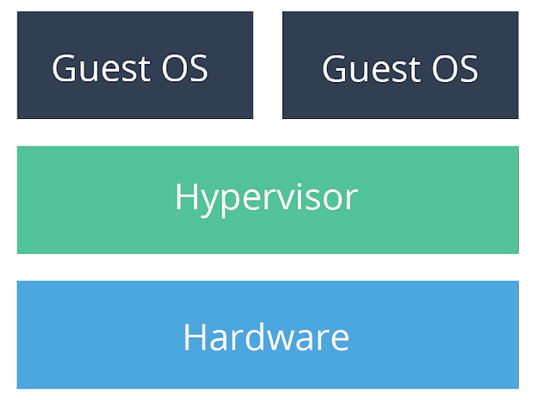
\includegraphics[width=0.7\linewidth]{images/Technologies/type_1_hypervisor.png}
	\caption{Type 1 (or bare metal) hypervisor architecture \cite{HypervisorsArchitectures}.}
	\label{fig:type_1_hypervisor}
\end{figure}

The greatest benefits of hypervisors are their robustness and scalability, enabling the efficient virtualization of large-scale applications and services.
However, the choice of creating a virtual machine using the Hyper-V Console Manager was dictated by two other reasons:

\begin{itemize}
	\item 
		The setup instructions described on the ebpf-for-windows GitHub repository tell the user to install a Windows virtual machine;
	\item 
		The so created isolated Windows 11 development environment provided a controlled space for testing and optimizing eBPF programs on the Windows platform.
		In fact, if anything goes wrong in this environment, we can just delete the virtual machine and create a new one, while if something bad happens in our host machine, we could break our computer.
\end{itemize}

So, to install eBPF on Windows the first thing that we have to do is to install our virtual machine.
To do so, we have to follow the instructions reported in the \textit{vm-setup.md} document \cite{WinVMSetupDoc}.
Besides the fact that that the virtual machine was configured with adequate resources to support development tasks effectively, the only thing worth noting is that during the quick creation of the virtual machine the option of \textit{Windows 11 dev environment} is the only one that can be selected since our host computer has Windows 11 as operative system (the tutorial tells to choose the \textit{Windows 10 dev environment} probably because, at the time of writing the document, version 10 of Windows was the highest available, but Windows 11 works as well).  

After the \textit{one-time setup} procedure is done, we have to decide how we are going to debug our virtual machine.
After a careful analysis of the requirements that we are going to need to make eBPF work, we decided to configure a kernel debugging connection over IP address.
In fact, since the eBPF for Windows binaries are not yet signed by Microsoft, they will only work on a machine with a kernel debugger attached and running or test signing is enabled.
Between the two, we decided to took the first route because it seemed easier and it will allow us to display some debug messages outside of the VM.
To do so there are a few articles on the \textit{Microsoft Learn} website, under the documentation section, that we have (once again) to follow by heart.
The two things that are worthy of note with this approach are the following:

\begin{itemize}
	\item 
		On our host computer we have to install a set of debugging tools for Windows.
		There are a few available \cite{DbgToolsWin}, but we decided to stick with the classic \textit{WinDbg}, a debugger that can be used to analyze crash dumps, debug live user-mode and kernel-mode code and examine CPU registers and memory \cite{InstallWinDbg}.
		After following the installation path of this tool, we will find it under \colorbox{backcolour}{\lstinline[style=commandline, language=bash, breaklines=true]|C:\\Program Files (x86)\\Windows Kits\\10\\Debuggers\\x64|};
	\item 
		Since it is very likely that sometimes we will shut down our virtual machine, every time that we are going to turn it on we have to start the kernel debugger attached to it (we will present later how to do it).
		This is quite inconvenient due to the fact that it requires a bit of time every time.  
\end{itemize}

At this point we have all the components that we will need on our host computer.
Now we have to install a series of applications on the virtual machine: under the \textit{Prerequisites} section of \textit{Building eBPF for Windows} in the \textit{GettingStarted.md} document \cite{GetStartDoc} there is a list of things to install in order to build the repository project.
Moreover, to make WinDbg work and debug the virtual machine over IP, we also have to install \textit{KDNET}, a debugging feature in Windows that allows remote kernel debugging over a network connection.

Once we have installed all the required tools, we are ready to start debugging our virtual machine.
With KDNET we have to set up the target machine (the one we want to debug) and the host machine (the one we will use for debugging) to communicate and then we can start the debugging session: an article on the Microsoft Learn websites tells us what to do \cite{SetUpNetDebug}.
However, even after we have followed all the listed steps the first time, whenever we want to turn on our virtual machine to work with eBPF, we have to redo some of these steps.
In particular, we have to:

\begin{itemize}
	\item 
		Open a \textit{Command prompt} with administrator privileges on both the machines;
	\item 
		Check the host IP address with the command \colorbox{backcolour}{\lstinline[style=commandline, language=bash, breaklines=true]|ipconfig|} because if we let the \textit{Dynamic Host Configuration Protocol} (\textit{DHCP}, a network management protocol used on IP networks for automatically assigning IP addresses and other communication parameters to devices connected to the network using a client–server architecture) to assign automatically an IP address to our computer, the address may vary;
	\item 
		On the virtual machine, in the \colorbox{backcolour}{\lstinline[style=commandline, language=bash, breaklines=true]|C:\\KDNET|} folder (that we should have created if we have correctly followed the last mentioned article), we have to run \colorbox{backcolour}{\lstinline[style=commandline, language=bash, breaklines=true]|kdnet <HostIPAddress> <DebugPort>|}, where the debug port must be within the range 50000-50039.
		This command will give us a few messages and another command that we have to copy and run on the host machine.
		It will look like this: \colorbox{backcolour}{\lstinline[style=commandline, language=bash, breaklines=true]|windbg -k net:port=<DebugPort>,key=<YourKey>|}, where the key consists of four alphanumeric strings separated by three dots;
	\item 
		On our host machine we have to:
		\begin{itemize}
			\item 
				Go to the folder where we have installed WinDbg, which is 
				
				\noindent
				\colorbox{backcolour}{\lstinline[style=commandline, language=bash, breaklines=true]|"C:\\Program Files (x86)\\Windows Kits\\10\\Debuggers\\x64"|};
			\item 
				Run the command that we have copied from the virtual machine.
		\end{itemize}
		After we have run the command, WinDbg will start on our host machine.
		However, for now, it says \textit{Debuggee not connected}.
		We have to do a couple more steps to make it work;
	\item 
		Disable \textit{Enhanced session} on the virtual machine using the \textit{View} pull down menu in the VM;
	\item 
		Restart the virtual machine with the command \colorbox{backcolour}{\lstinline[style=commandline, language=bash, breaklines=true]|shutdown -r -t|}.
		If after we restart the virtual machine one time the \textit{Debuggee not connected} string did not change, we have to restart it a second time.
		If we do so, we should be able to see \textit{Debugger is running...}.
\end{itemize}

After everything is done we now have started our virtual machine with a kernel debugger attached.
In Figure \ref{fig:WinDbg} we can look at what we should see once we start the Windows debugger on our host machine.
In particular, Figure \ref{fig:WinDbgNc} shows the debugger interface immediately after we run the \colorbox{backcolour}{\lstinline[style=commandline, language=bash, breaklines=true]|windbg|} command on our host machine, while Figure \ref{fig:WinDbgR} displays the interface once we reboot our virtual machine two times.

\begin{figure}[h]
	\centering
	\begin{subfigure}{.5\textwidth}
		\centering
		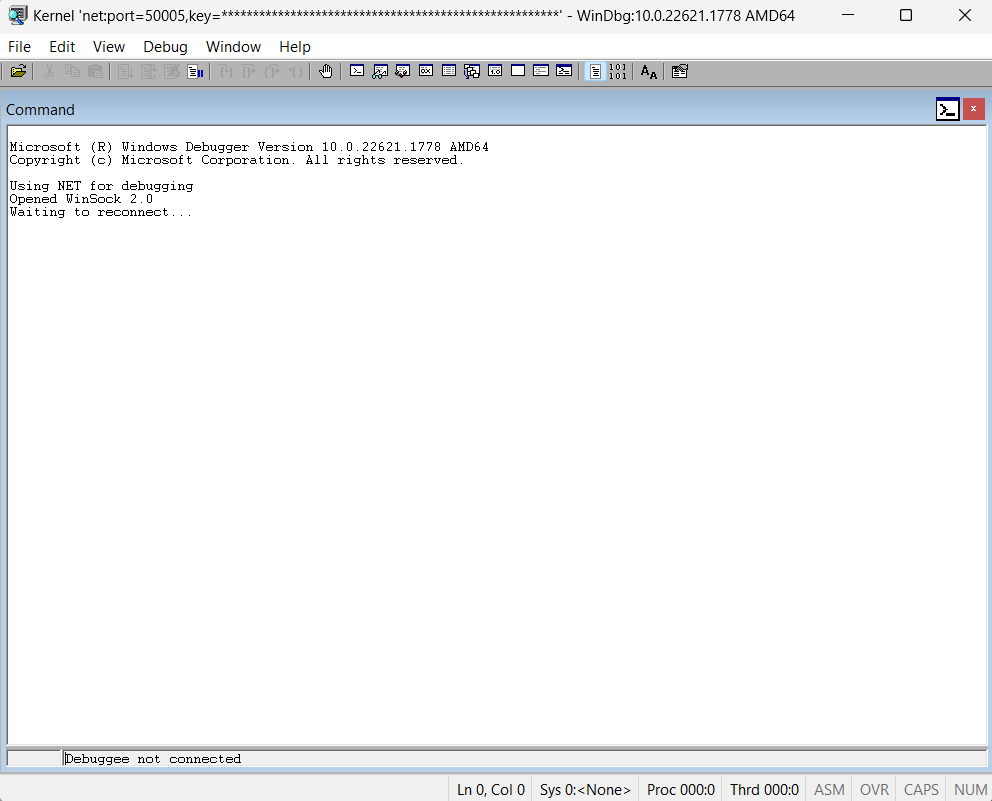
\includegraphics[width=0.9\linewidth]{images/WindowsDevelopment/WinDbg_nc.png}
		\caption{}
		\label{fig:WinDbgNc}
	\end{subfigure}%
	\begin{subfigure}{.5\textwidth}
		\centering
		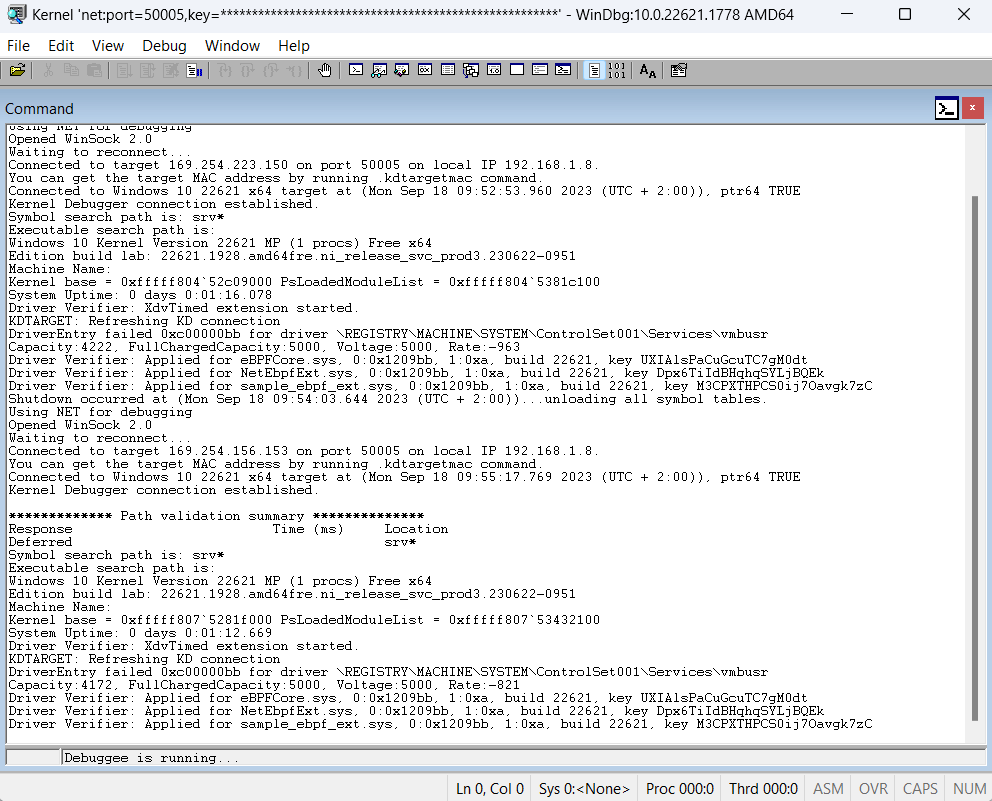
\includegraphics[width=0.9\linewidth]{images/WindowsDevelopment/WinDbg_r.png}
		\caption{}
		\label{fig:WinDbgR}
	\end{subfigure}	
	\caption{Windows debugger interface: (a) after starting WinDbg on our host machine; (b) after rebooting the virtual machine twice.}
	\label{fig:WinDbg}
\end{figure}

Note that this process must be done every time we want to turn on the virtual machine to work with eBPF.
Even if the IP address of our computer or the debug port change, the command that we have to run to start WinDbg on our host machine will always be the some.
However, if we do not go through the kdnet procedure on our virtual machine, the debugger will never get attached to it.

At this point, remember to do the last point on the vm-setup.md document which is \textit{Enable Driver Verifier on eBPF drivers}.

The last step that we have to make is to install ebpf-for-windows.
To do so, we have to follow the instructions given by the \textit{InstallEbpf.md} document \cite{InseBPFDoc}.
The easiest way to install eBPF into a test virtual machine is to stick to the so called \textit{Method 1}.
For this thesis we worked with the \textit{v0.9.0} version, but, at the time of writing, versions \textit{v0.10.0} and \textit{v0.11.0} were released.
We can understand how fast this technology is evolving on Windows.

Once we have done with all the set up part, we can now start developing some examples using the ebpf-for-windows project.
We must point out that from now on we will assume that we are working on a virtual machine that has been turned on with a kernel debugger attached, as we explained previously.

\section{How to use eBPF on Windows}

To develop eBPF applications on Linux we used two projects that made this task relatively simple once we understood the logic behind eBPF.
Unfortunately, with ebpf-for-windows this doesn't happen.
However, the repository provides several documents in which it explains how to develop simple initial programs and how to debug them.

Before diving into that, we have to build our project: to do so, we have to follow the \textit{How to clone and build the project using Visual Studio} section in the GettingStarted.md document which consists of some operations besides cloning the repository.
After a series of attempts, we suggest to build the project by following the instructions given for \textit{Developer Command Prompt for VS 2022} because we could not figure out how to perform this task with \textit{Visual Studio IDE} since during the process we get some error messages.
After a few minutes, the process comes to an end and we have successfully built the project (there would probably be some warnings, but we can ignore them).

Now, we can finally start writing some eBPF programs.
We warmly invite the users new to eBPF on Windows (even the ones with plenty of experience with eBPF on Linux) to do the basic tutorial that can be found in the \textit{tutorial.md} document \cite{TutDoc}.
The complexity of the programs is really low, but the examples are very useful for understanding the outputs of a series of terminal commands regarding eBPF which in turn explain the programs' structure.

Even though the tutorial is pretty clear, we have to point out a few things to give a full perspective of writing an eBPF program on Windows:

\begin{itemize}
	\item 
		To explain how sections work, the tutorial first uses \colorbox{backcolour}{\lstinline[style=commandline, language=bash, breaklines=true]|#pragma clang section|} and then switches to the macro \colorbox{backcolour}{\lstinline[style=commandline, language=bash, breaklines=true]|SEC("...")|}.
		They have the same effect, but we suggest to stick to the traditional way that we have already seen in Linux; 
	\item 
		From the tutorial we can see that inside the \colorbox{backcolour}{\lstinline[style=commandline, language=bash, breaklines=true]|SEC("...")|} macro we could write anything we want.
		However, the number of valid hook points is limited (and they are different from Linux).
		To see what are the strings that can be written inside the macro to designate which hook point the eBPF program is designed for, we have to run \colorbox{backcolour}{\lstinline[style=commandline, language=bash, breaklines=true]|ls HKCU:\\Software\\eBPF\\Providers\\SectionData|} on \textit{Windows PowerShell} (not Command Prompt) terminal with administrator privileges;
	\item 
		Among all the examples provided by the tutorial, not all of them can be installed inside the Windows kernel.
		If we want to do so, inside the \colorbox{backcolour}{\lstinline[style=commandline, language=bash, breaklines=true]|SEC("...")|} macro we must use a string for a valid hook point;
	\item 
		If we attempt to include an header file, during the compilation process of our program we could get an error indicating that the file has not been found.
		We can resolve this by specifying the full path to that file (in our case, for example, to include the \colorbox{backcolour}{\lstinline[style=commandline, language=bash, breaklines=true]|bpf_helpers.h|} header in our programs, we should write\\\colorbox{backcolour}{\lstinline[style=commandline, language=bash, breaklines=true]|#include "C:\\eBPF-for-Windows.0.9.0\\build\\native\\include\\bpf_helpers.h"|}.
\end{itemize}

Once we are done with the basic tutorial, there is a more complex one that illustrates how to understand and debug eBPF verification failures in the \textit{debugging.md} document \cite{DebugDoc}.
We are not going to cover it since our focus is to take the developed programs, install them inside the kernel, make them run and read some output strings.

In fact, now we are going to develop our first program: like we did in Linux, we are going to write a simple \textit{Hello World!}-like program and we are going to show all the process required to look at some debug messages.

In Windows we have just to define the code of the program that we are going to inject in the kernel: we will call our program \colorbox{backcolour}{\lstinline[style=commandline, language=bash, breaklines=true]|helloworld.c|}.

However, once we try to write some code (for example using Visual Studio), in our kernel debugger on our host machine several error messages will appear:

\begin{lstlisting}[style=commandline, language=bash, caption={Windows kernel debugger error messages.}]
	WER/CrashAPI:2693: ERROR Invalid args, too  big block
	WER/CrashAPI:2882: ERROR PEB is not initialized
\end{lstlisting}

We can just ignore them: for the purpose of this thesis we have not studied the debugger in depth, but there is a lot about it in the documentation on Microsoft Learn.
We will see later that our debugger works and prints debug messages.

In the following there is the code of our \colorbox{backcolour}{\lstinline[style=commandline, language=bash, breaklines=true]|helloworld.c|} program.

\begin{lstlisting}[style=cstyle, language=C, caption={Code of the ``Hello world!''-like kernel side program in ebpf-for-windows.}, title=helloworld.c]
	#include "C:\\eBPF-for-Windows.0.9.0\\build\\native\\include\\bpf_helpers.h|"
	
	SEC("xdp")
	int print_helloworld(xdp_md_t *ctx) {
		int n = bpf_get_prandom_u32();
		bpf_printk("Hello World %d!", n);
		return 0;
	}
\end{lstlisting}

Looking at the code, there are a few things that we have to point at because they are different from Linux:

\begin{itemize}
	\item 
		There is no need to define a \colorbox{backcolour}{\lstinline[style=commandline, language=bash, breaklines=true]|LICENSE|} for our eBPF code;
	\item 
		As we mentioned earlier, we can now see that to include an header file for working with eBPF we have to include all the path to that file;
	\item 
		For this simple example we wanted to use two of the helpers provided for Windows.
		The full documentation about eBPF API for Windows can be found on GitHub \cite{eBPFWinDoc};
	\item 
		We decided to use the \colorbox{backcolour}{\lstinline[style=commandline, language=bash, breaklines=true]|xdp|} hook point which defines a section meant as an XDP layer program.
		In other words, every time network packets are exchanged (for example, by searching something on the browser), the program is triggered.
\end{itemize}

The logic behind the program is very simple: first, it gets a random number from \colorbox{backcolour}{\lstinline[style=commandline, language=bash, breaklines=true]|bpf_get_prandom_u32()|} and then prints a string with \colorbox{backcolour}{\lstinline[style=commandline, language=bash, breaklines=true]|bpf_printk()|} using the previously generated number as parameter.
If we had tried to do the printing of a message like we did in Linux (i.e. defining a string variable and printing it), the program would fail the process of compilation because, as the time of writing, \colorbox{backcolour}{\lstinline[style=commandline, language=bash, breaklines=true]|bpf_printk()|} can just print the standard string given as first parameter and can accept from zero to a maximum of three numbers as other parameters.

Once we have written our program we are ready to inject it into the kernel.
To do so, we have to work from Command Prompt with administrator privileges.
As we learned from the tutorial.md document, first we have to compile our program with Clang:

\begin{lstlisting}[style=commandline, language=bash, caption={``Hello world!''-like program compilation command in ebpf-for-windows.}]
	clang -target bpf -Werror -g -O2 -c helloworld.c -o helloworld.o
\end{lstlisting}

The important options of this command are \colorbox{backcolour}{\lstinline[style=commandline, language=bash, breaklines=true]|-Werror|}, that specifies that warnings are errors, \colorbox{backcolour}{\lstinline[style=commandline, language=bash, breaklines=true]|-02|}, which is for compiling an optimized build and \colorbox{backcolour}{\lstinline[style=commandline, language=bash, breaklines=true]|-g|} which keeps the symbol information.
We will not cover all the possible commands that the tutorial presented.
The curious users can look deeper into the characteristics of this program using the other commands.

Then we have to install this program into the kernel with the following command.

\begin{lstlisting}[style=commandline, language=bash, caption={``Hello world!''-like program installation command in ebpf-for-windows.}]
	netsh ebpf add program helloworld.o
\end{lstlisting}

If the loading of the program into the kernel is successful we will get in return a program ID associated to it.
However, we have to mention a major problem that we faced when we were loading programs into the kernel.
To perform network debugging we have to create a \textit{virtual network adapter} (\textit{vNIC}) to emulate the behavior of a physical network adapter in order to provide network connectivity to our virtual machine.
However, since we are loading a program which has \colorbox{backcolour}{\lstinline[style=commandline, language=bash, breaklines=true]|xdp|} as hook point, our virtual machine loses network connectivity every time we load our \colorbox{backcolour}{\lstinline[style=commandline, language=bash, breaklines=true]|helloworld.c|} program in the kernel and regains it every time we remove it from the kernel.
This will also happen with all the other hook points that are shown in the repository since they are all related to networking: in fact, as the time of writing, Windows does not provide many hook points (for example, there is no \colorbox{backcolour}{\lstinline[style=commandline, language=bash, breaklines=true]|execve|} hook point like in Linux) and the ones available are not well-documented.
Inside the \textit{Settings} of our virtual machine we will display the following message:

\begin{lstlisting}[style=commandline, language=bash, caption={Network adapter problem message on the virtual machine.}]
	You're connected using a virtual network adapter that we can't test.
\end{lstlisting}

This means that we could not browse in the internet in our virtual machine.
However, we will be able to watch debug messages anyway (but we could not figure out why).

Once the program is injected into the kernel, we are now ready to see some output strings.
In the GettingStarted.md document, under the section \textit{Using tracing}, there is an explanation on how we can look at some debugging output.
eBPF on Windows uses \textit{Event Tracing for Windows} for logging traces: to view traces in real-time, the  \colorbox{backcolour}{\lstinline[style=commandline, language=bash, breaklines=true]|tracelog.exe|} and \colorbox{backcolour}{\lstinline[style=commandline, language=bash, breaklines=true]|tracefmt.exe|} commands from the \textit{Windows Driver Kit} (\textit{WDK}, a set of software tools from Microsoft that enables the development of device drivers for the Microsoft Windows platform that we were told to install in the in the Prerequisites section in the GettingStarted.md document) can be used.  
However, there is another very interesting way to do so, depending on where we want to generate our output.

If we want to see our debug strings in the Command Prompt in real time we have to follow the instruction on the document mentioned above.
In particular, in another Command Prompt with administrator privileges, we have to type in the following commands:

\begin{lstlisting}[style=commandline, language=bash, caption={Commands to start real-time debugging using \colorbox{backcolour}{\lstinline[style=commandline, language=bash]|tracelog|} and \colorbox{backcolour}{\lstinline[style=commandline, language=bash]|tracefmt|}.}]
	cd C:\\Program Files (x86)\\Windows Kits\\10\\bin\\10.0.22621.0\\x64
	tracelog -start MyTrace -guid "%ProgramFiles%\[eBPF for Windows install folder]\ebpf-printk.guid" -rt 
	tracefmt -rt MyTrace -displayonly -jsonMeta 0
	tracelog -stop MyTrace
\end{lstlisting}

This is an important part of this process, so we have to be very careful about it:

\begin{itemize}
	\item 
		The first command brings in a folder where we can find the \colorbox{backcolour}{\lstinline[style=commandline, language=bash, breaklines=true]|tracelog|} and the \colorbox{backcolour}{\lstinline[style=commandline, language=bash, breaklines=true]|tracefmt|} programs that we are going to use to print our debug output;
	\item 
		The second command creates the trace session, a period during which a process is generating trace messages.
		Instead of \colorbox{backcolour}{\lstinline[style=commandline, language=bash, breaklines=true]|[eBPF for Windows install folder]|} we had to put our path to that folder: since in our case it was located in \colorbox{backcolour}{\lstinline[style=commandline, language=bash, breaklines=true]|C:\\Program Files\\ebpf-for-windows|}, we just had to replace the string between brackets with \colorbox{backcolour}{\lstinline[style=commandline, language=bash, breaklines=true]|ebpf-for-windows|}.
		Moreover, we just want to look at the output printed by \colorbox{backcolour}{\lstinline[style=commandline, language=bash, breaklines=true]|bpf_printk()|}, so we specified the \colorbox{backcolour}{\lstinline[style=commandline, language=bash, breaklines=true]|ebpf-printk.guid|} file in the command.
		However, we could look at all sort of messages if we replace it with \colorbox{backcolour}{\lstinline[style=commandline, language=bash, breaklines=true]|ebpf-all.guid|};
	\item 
		The third command lets us view the tracing session in real time on terminal;
	\item 
		The last command closes the trace session.
\end{itemize}

After running the first three commands, every time that the program triggers, we will get a new string on our Command Prompt that should look like this:

\begin{lstlisting}[style=commandline, language=bash, caption={Real-time output messages format using \colorbox{backcolour}{\lstinline[style=commandline, language=bash]|tracelog|} and \colorbox{backcolour}{\lstinline[style=commandline, language=bash]|tracefmt|}.}]
	[CPU_ID]process_ID.thread_ID::gg/mm/yyyy-hh:mm:ss.sss [EbpfForWindowsProvider]{"Message":"Hello World x!"}
\end{lstlisting}

Apart from the IDs (the CPU one is just a number, while the process and the thread ones are in hexadecimal) and the date and time information, at the end we get our debugging message (\colorbox{backcolour}{\lstinline[style=commandline, language=bash, breaklines=true]|x|} is the number generated randomly which varies in each message).
Once we are done with the tracing session, we press \colorbox{backcolour}{\lstinline[style=commandline, language=bash, breaklines=true]|CTRL+C|} to interrupt the execution of the \colorbox{backcolour}{\lstinline[style=commandline, language=bash, breaklines=true]|tracefmt|} command.
Then, we run the last command to stop the tracing session: if we do not do this, we will not be able to start a new tracing session with the same name using the \colorbox{backcolour}{\lstinline[style=commandline, language=bash, breaklines=true]|tracelog|} command.

However, once we close our terminal, all the information that we got from our tracing session gets lost.
On Windows there is a way to save all the debug messages in a file (and this cannot be done on Linux).
The process is similar to before, but this time the commands that we have to run are the following:

\begin{lstlisting}[style=commandline, language=bash, caption={Commands for kernel debugging using \colorbox{backcolour}{\lstinline[style=commandline, language=bash]|tracelog|}.}]
	cd C:\\Program Files (x86)\\Windows Kits\\10\\bin\\10.0.22621.0\\x64
	tracelog -start MyTrace -guid "%ProgramFiles%\[eBPF for Windows install folder]\ebpf-printk.guid" -kd
	tracelog -stop MyTrace
	netsh trace convert LogFile.Etl Output.csv csv
\end{lstlisting}

There are a few important things to look at:

\begin{itemize}
	\item 
		The first command is the same as before;
	\item 
		The second command does the same thing as before, but it has \colorbox{backcolour}{\lstinline[style=commandline, language=bash, breaklines=true]|-kd|} instead of \colorbox{backcolour}{\lstinline[style=commandline, language=bash, breaklines=true]|-rt|} at its end: this changes everything.
		In fact, now we can see the output messages in two different places:
		\begin{itemize}
			\item 
				In the kernel debugger interface;
			\item 
				In a \colorbox{backcolour}{\lstinline[style=commandline, language=bash, breaklines=true]|LogFile.Etl|} which can be found in the same directory as \colorbox{backcolour}{\lstinline[style=commandline, language=bash, breaklines=true]|tracelog|} (i.e. \colorbox{backcolour}{\lstinline[style=commandline, language=bash, breaklines=true]|C:\\Program Files (x86)\\Windows Kits\\10\\bin\\10.0.22621.0\\x64|}).
		\end{itemize}
		Now, every time the program gets triggered, on the kernel debugger interface a new message gets printed and the \colorbox{backcolour}{\lstinline[style=commandline, language=bash, breaklines=true]|LogFile.Etl|} gets updated.
		It is a bit like before where in Command Prompt new debug messages were printed in real time, but now they are printed in different locations;
	\item 
		The third command works in the same way as before;
	\item 
		The last command is a new one and we used it to transform the \colorbox{backcolour}{\lstinline[style=commandline, language=bash, breaklines=true]|Etl|} file generated by \colorbox{backcolour}{\lstinline[style=commandline, language=bash, breaklines=true]|tracelog|} in a \colorbox{backcolour}{\lstinline[style=commandline, language=bash, breaklines=true]|csv|} file to make it readable.
		This file has as many rows as the number of debug messages generated by our program and quite a few columns which contain different information about our messages and we can find it in the same directory of the \colorbox{backcolour}{\lstinline[style=commandline, language=bash, breaklines=true]|Etl|} file.
\end{itemize}

In the kernel debugger interface the printed messages have a very similar structure as the ones printed in Command Prompt with the previous sequence of commands:

\begin{lstlisting}[style=commandline, language=bash, caption={Kernel debugging output messages format using \colorbox{backcolour}{\lstinline[style=commandline, language=bash]|tracelog|}.}]
	[CPU_ID]process_ID.thread_ID::gg/mm/yyyy-hh:mm:ss.sss [EbpfForWindowsProvider/EbpfGenericMessage]{"Message":"Hello World x!"}
\end{lstlisting}

In addition we have the information about the event name which, in this case, is \colorbox{backcolour}{\lstinline[style=commandline, language=bash, breaklines=true]|EbpfGenericMessage|}.

Instead, in the \colorbox{backcolour}{\lstinline[style=commandline, language=bash, breaklines=true]|csv|} file all the information is disposed into columns: we can find the event name, the process ID, the date and time, the user data (which contains just our \colorbox{backcolour}{\lstinline[style=commandline, language=bash, breaklines=true]|Hello World x!|} message) and many more. 

These are two ways to perform debugging with \colorbox{backcolour}{\lstinline[style=commandline, language=bash, breaklines=true]|bpf_printk()|} on Windows.
Once we are done with the tracing session, we must remember to remove the program from where we have installed it with the following command:

\begin{lstlisting}[style=commandline, language=bash, caption={``Hello world!''-like program delete command in ebpf-for-windows.}]
	netsh ebpf delete program program_id
\end{lstlisting}

In this case, the \colorbox{backcolour}{\lstinline[style=commandline, language=bash, breaklines=true]|program_id|} is the one that we get in return when we installed the program.

\section{The windows-ebpf-starter project}

At this point we have understood how to work with eBPF on Windows.
However, we can clearly see that the procedure that we have to do every time to get some information about our program is quite long and complex.
If we make a comparison between what the projects that we have seen in Linux (i.e. BumbleBee and libbpf-bootstrap) and ebpf-for-windows, the second loses due to the difficulty of use.

Luckily, during our research, we came across an article written in a blog of an Indian IT company founded in 2020 that works on security for distributed devices and data called \textit{Subconscious Compute} \cite{SubComWebsite}.
In this article, published at the beginning of 2023, the author Gurnoor Virdi, who made an internship with them, talks about eBPF programming on Windows \cite{eBPFWinSubComBlogArticle}: he covers the topics of installation and programming model of eBPF (which we have already discussed in the previous paragraph) and, most importantly for us, talks about an environment that, after a first reading, looks similar to libbpf-bootstrap.

However, the virtual machine setup and the installation of the eBPF runtime (what we get after we follow the Method 1 in the InstallEbpf.md document of the ebpf-for-windows repository) have to be performed anyway if we want to run an eBPF program.
So, once again, we will take for granted that the virtual machine has been turned on with a kernel debugger attached.

Now that everything is set up we can start working on the environment described in the article.
Unfortunately, the repository that is mentioned in the document is on \textit{GitLab}, another open source web platform used to manage Git repositories, and only the Subconscious Compute users have access to it.
However, we wrote them an email asking if they could give us access to that repository and they replied saying that they would put the repository on GitHub and make it open source under AGPL license: the project is called \textit{windows-ebpf-starter} \cite{WineBPFStarterRepo}.

After we cloned the repository on our virtual machine, we built the environment by following the instructions on the article and did the tutorial about \textit{Writing and compiling a simple eBPF program}.
Once we became familiar with the environment, we decided to reproduce the same examples that we did in Linux to make a fair comparison between two programs that should do the same thing.
For this purpose, in the following we are going to present a program very similar to the one that used an \colorbox{backcolour}{\lstinline[style=commandline, language=bash, breaklines=true]|HashMap|}: we will call it \colorbox{backcolour}{\lstinline[style=commandline, language=bash, breaklines=true]|hash_map_use.c|}

\begin{lstlisting}[style=cstyle, language=C, caption={Code of the program that uses a map in windows-ebpf-starter.}, title=hash\_map\_use.c]
	#include "stdint.h"
	#include "bpf_helpers.h"
	#include "bpf_helper_defs.h"
	#include "ebpf_structs.h"
	
	SEC("maps")
	ebpf_map_definition_in_file_t hash_map = {
		.type = BPF_MAP_TYPE_HASH,
		.max_entries = 256 * 1024,
		.key_size = sizeof(uint64_t),
		.value_size = sizeof(int64_t),
	};
	
	static void hash_map_use(uint64_t pid, uint64_t time_stamp){
		bpf_printk("### BEGIN HASH MAP USE ###");
		
		int64_t update;
		int64_t delete;
		
		uint64_t *found;
		uint64_t *deleted;
		
		update = bpf_map_update_elem(&hash_map, &pid, &time_stamp, EBPF_ANY);
		
		bpf_printk("UPDATE: pid %d - update %d.", pid, update);
		
		bpf_printk("key pid %d - ts %llu - update %d.", pid, time_stamp, update);
		
		found = (uint64_t *) bpf_map_lookup_elem(&hash_map, &pid);
		
		if (found) {
			bpf_printk("FOUND IN HASH MAP: pid %d - *found %llu.", pid, *found);
		} else {
			bpf_printk("NOT FOUND IN HASH MAP");
		}
		
		delete = bpf_map_delete_elem(&hash_map, &pid);
		
		bpf_printk("DELETE: pid %d - delete %lld.", pid, delete);
		
		deleted = (uint64_t *)bpf_map_lookup_elem(&hash_map, &pid);
		
		if (deleted) {
			bpf_printk("DELETED IN HASH MAP: pid %d - *deleted %llu).", pid, *deleted);
		} else {
			bpf_printk("NOT DELETED IN HASH MAP.");
		}
		
		bpf_printk("### END HASH MAP USE ###\n\n");
	}
	
	SEC("xdp")
	int print_pid_hash_map(xdp_md_t* ctx)
	{
		uint64_t pid;
		uint64_t time_stamp;
		
		pid = bpf_get_current_pid_tgid() >> 32;
		time_stamp = bpf_ktime_get_ns(); 
		
		bpf_printk("BPF triggered from PID %d at time %llu.\n", pid, time_stamp);
		
		hash_map_use(pid, time_stamp);
		
		return 0;
	}
\end{lstlisting}

Apart from the different way of defining an eBPF map and some types of some variables, the logic of the program is the same as the program in Linux: 

\begin{itemize}
	\item 
		Take the process ID with \colorbox{backcolour}{\lstinline[style=commandline, language=bash, breaklines=true]|bpf_get_current_pid_tgid() >>32|} and the time from system boot with \colorbox{backcolour}{\lstinline[style=commandline, language=bash, breaklines=true]|bpf_ktime_get_ns()|} and pass them by copy to the sub-program \colorbox{backcolour}{\lstinline[style=commandline, language=bash, breaklines=true]|hash_map_use()|};
	\item 
		Add them to the \colorbox{backcolour}{\lstinline[style=commandline, language=bash, breaklines=true]|HashMap|} with the \colorbox{backcolour}{\lstinline[style=commandline, language=bash, breaklines=true]|pid|} as key and the \colorbox{backcolour}{\lstinline[style=commandline, language=bash, breaklines=true]|time_stamp|} as value;
	\item 
		Look for the \colorbox{backcolour}{\lstinline[style=commandline, language=bash, breaklines=true]|pid|} value in the map (which will always be found);
	\item 
		Delete the \colorbox{backcolour}{\lstinline[style=commandline, language=bash, breaklines=true]|pid|}-\colorbox{backcolour}{\lstinline[style=commandline, language=bash, breaklines=true]|time_stamp|} couple from the map;
	\item 
		Check if the delete operation has been done successfully by looking again for the \colorbox{backcolour}{\lstinline[style=commandline, language=bash, breaklines=true]|pid|} value in the map.
\end{itemize}

Once we compile the program with the \colorbox{backcolour}{\lstinline[style=commandline, language=bash, breaklines=true]|build.bat|} file provided by the project, we can then load it into the kernel and start a tracing session with \colorbox{backcolour}{\lstinline[style=commandline, language=bash, breaklines=true]|tracelog|}, following the one of the two procedures that we have seen earlier.

After doing so, we will see the following output:

\begin{lstlisting}[style=commandline, language=bash, caption={Debug messages of the program that uses a map in windows-ebpf-starter.}]
	"BPF triggered from PID ``pid'' at time ``time_stamp''."
	"### BEGIN HASH MAP USE ###"
	"UPDATE: pid ``pid'' - update 0."
	"key pid ``pid'' - ts ``time_stamp'' - update 0."
	"FOUND IN HASH MAP: pid ``pid'' - *found ``time_stamp''."
	"DELETE: pid ``pid'' - delete 0."
	"NOT DELETED IN HASH MAP."
	"### END HASH MAP USE ###"
\end{lstlisting}

There are a few interesting things about this output messages:

\begin{itemize}
	\item 
		We did report just the debug messages, omitting the information about the process and thread IDs, the date and time and the CPU number;
	\item 
		As the output of the Linux program, \colorbox{backcolour}{\lstinline[style=commandline, language=bash, breaklines=true]|pid|} and \colorbox{backcolour}{\lstinline[style=commandline, language=bash, breaklines=true]|time_stamp|} are between quotes because they depend on the particular execution of the program;
	\item 
		Due to the problem with the virtual network adapter that we have discussed previously, the process ID will always be 0, meaning that the system is in idle.
		However, this is not important if we just want to show how this program works;
	\item 
		The second-to-last message suggests that the delete operation has not been performed successfully, even though the \colorbox{backcolour}{\lstinline[style=commandline, language=bash, breaklines=true]|bpf_map_delete_elem()|} returns 0.
		We could not figure out why this happens, so we tried to develop the exact same program using an \colorbox{backcolour}{\lstinline[style=commandline, language=bash, breaklines=true]|ArrayMap|} instead of the \colorbox{backcolour}{\lstinline[style=commandline, language=bash, breaklines=true]|HashMap|}.
		The result was interesting: all the debug messages were the same except for the penultimate one, which was \colorbox{backcolour}{\lstinline[style=commandline, language=bash, breaklines=true]|"DELETED IN ARRAY: pid ``pid'' - *deleted 0."|}.
		It looks like that the delete method works well with the \colorbox{backcolour}{\lstinline[style=commandline, language=bash, breaklines=true]|ArrayMap|}, but gives some problems with the \colorbox{backcolour}{\lstinline[style=commandline, language=bash, breaklines=true]|HashMap|};
	\item 
		We remember that with \colorbox{backcolour}{\lstinline[style=commandline, language=bash, breaklines=true]|bpf_printk()|} we can just print numbers on Windows, so we could not print the \colorbox{backcolour}{\lstinline[style=commandline, language=bash, breaklines=true]|deleted|} pointer to see its value and understand what goes wrong in the delete operation.
\end{itemize}

Besides learning some new things about eBPF maps, it seems that this project, which we looked at with hope, does not significantly simplify things when we have to load a program inside the kernel and look at some debug output.
It makes the process of compilation easier because it defines the \colorbox{backcolour}{\lstinline[style=commandline, language=bash, breaklines=true]|build.bat|} file which allows us to compile multiple programs at once, but other than that we have to use again the commands that are shown in the tutorial.md document in the ebpf-for-windows repository.

However, the article of Gurnoor Virdi does not stop with the writing of some simple eBPF programs: the section called \textit{Working with userspace} is the most interesting part about this project because it shows how we can manage the lifetime of an eBPF program through an user space application (like we did with libbpf-bootstrap).

The idea is the same of the one that we have already seen in Linux: create a user space application that uses a series of methods to manage the various phases that an eBPF kernel side program goes through: opening, loading, attaching and unloading.
However, these methods are not automatically generated in a skeleton file by the environment after the compilation of the kernel source code of the program that we want to control from user space: they are defined in an header file inside the eBPF runtime, called \colorbox{backcolour}{\lstinline[style=commandline, language=bash, breaklines=true]|libbpf.h|}, which can be found in the the \colorbox{backcolour}{\lstinline[style=commandline, language=bash, breaklines=true]|..\\ebpf-for-windows.0.9.0\\build\\native\\include\\libbpf\\src|} folder (the documentation of this header can be found in a page of the eBPF for Windows documentation on GitHub \cite{eBPFWinlibbpfHeader}).
In fact, we only need two things to make the user space application work:

\begin{itemize}
	\item 
		The path to the object file (which has \colorbox{backcolour}{\lstinline[style=commandline, language=bash, breaklines=true]|.o|} extension) generated from the kernel source code after the process of compilation;
	\item 
		The name of the eBPF program that we want to load into the kernel (in other words, the name of the function defined after \colorbox{backcolour}{\lstinline[style=commandline, language=bash, breaklines=true]|SEC("hook_point")|}).
\end{itemize}

Once we have these 2 things we can use the \colorbox{backcolour}{\lstinline[style=commandline, language=bash, breaklines=true]|bpf_object__open()|} method to create a pointer to a \colorbox{backcolour}{\lstinline[style=commandline, language=bash, breaklines=true]|bpf_object|}, which we are going to use in the following phases as a parameter of other methods, such as \colorbox{backcolour}{\lstinline[style=commandline, language=bash, breaklines=true]|bpf_object__load()|} to load the object code into the kernel, \colorbox{backcolour}{\lstinline[style=commandline, language=bash, breaklines=true]|bpf_object__attach()|} to attach the program to an hook point and \colorbox{backcolour}{\lstinline[style=commandline, language=bash, breaklines=true]|bpf_object__close()|} to unload the object code from the kernel.

However, we tried to do the tutorial described in the article, but we could not manage to correctly compile the user space application.
Every time we get a fatal error saying that the  \colorbox{backcolour}{\lstinline[style=commandline, language=bash, breaklines=true]|\#include|} files cannot be found.
In particular, we get the \colorbox{backcolour}{\lstinline[style=commandline, language=bash, breaklines=true]|0x2|} error code which corresponds to \colorbox{backcolour}{\lstinline[style=commandline, language=bash, breaklines=true]|ERROR_FILE_NOT_FOUND|}. 
This error code indicates that the system or a program attempted to perform an operation on a file or directory that does not exist at the specified location.

We get this error for including all the headers, but for different reasons:

\begin{itemize}
	\item 
		If we include a standard C library (such as \colorbox{backcolour}{\lstinline[style=commandline, language=bash, breaklines=true]|iostream|}), the compiler says that it cannot find such file;
	\item 
		If we include an header file from the eBPF runtime (such as \colorbox{backcolour}{\lstinline[style=commandline, language=bash, breaklines=true]|libbpf.h|}), even if we put the full path to that file the compiler says that he cannot find some other headers.
		In fact, in the header files of the eBPF runtime, there are plenty of \colorbox{backcolour}{\lstinline[style=commandline, language=bash, breaklines=true]|\#include|} of some other header files.
\end{itemize}

We think that the problem is the way in which the project is structured: in the tutorial we are told to modify the \colorbox{backcolour}{\lstinline[style=commandline, language=bash, breaklines=true]|Makefile|} and add our particular paths to the location of the include directory of the eBPF development files we downloaded through the \colorbox{backcolour}{\lstinline[style=commandline, language=bash, breaklines=true]|nuget|} package (i.e. \colorbox{backcolour}{\lstinline[style=commandline, language=bash, breaklines=true]|..\\ebpf-for-windows.0.9.0\\build\\native\\include|}) and to the location of the lib directory containing \colorbox{backcolour}{\lstinline[style=commandline, language=bash, breaklines=true]|EbpfApi.lib|} from the eBPF install directory (i.e. \colorbox{backcolour}{\lstinline[style=commandline, language=bash, breaklines=true]|..\\ebpf-for-windows.0.9.0\\build\\native\\lib|}).
We think that this tells the compiler to look for all the files that we include in our user space program just in the first of these two folders, but, obviously, not all headers are in that exact directory.

So, although windows-ebof-starter looks very promising, we were only able to make it work with the kernel side code and the commands that are reported in the tutorial.md document in ebpf-for-windows.


\chapter{Conclusions}

This master's thesis has provided a comprehensive exploration of Extended Berkeley Packet Filter (eBPF), a transformative technology reshaping the landscape of networking, observability, and security in modern computing. 
Our study encompassed an in-depth examination of its historical evolution, intricate toolchain, versatile ecosystem and development aspects, with a particular focus on its presence and impact across both the Linux and Windows platforms.

The historical evolution of eBPF was traced, beginning with its origins in the Berkeley Packet Filter (BPF) and its subsequent evolution into eBPF. 
This journey highlighted how eBPF's flexible design enabled it to go beyond its initial networking-centric role, finding applications in diverse areas such as observability and security.

We delved into the complexities of the eBPF toolchain, revealing a sophisticated process that involves program development in languages like C, followed by compilation, verification and Just-In-Time (JIT) compilation into native kernel code.
This marked eBPF's power and efficiency as a tool for extending kernel capabilities.

Then, the eBPF ecosystem was explored, emphasizing the significance of key components like maps for efficient data exchange and helpers for smooth interaction with the kernel.
These elements collectively constitute a robust toolkit for eBPF program development.

Our investigation into eBPF program development highlighted its event-driven nature, allowing for the interception of system calls, function tracing and network traffic analysis, all without the need for kernel recompilation.

Furthermore, it is important to note that eBPF technology is still undergoing significant development. 
Moreover, its adoption and synchronization between Linux and Windows platforms are not fully aligned, as one platform's implementation preceded the other.

In the Linux community, we anticipate accelerated development of new eBPF tools, libraries and frameworks, expanding its utility into domains like Internet of Things (IoT) and edge computing.

Within the Windows domain, eBPF is at the edge of becoming widely adopted and essential in various software applications, particularly in areas like network monitoring, security enforcement, and performance optimization, because more and more projects are recognizing its potential and starting to incorporate it into their solutions.

In summation, eBPF represents a remarkable evolution in systems programming, fundamentally altering our interaction with and understanding of modern computing environments. 
As eBPF continues to evolve, it is certain that it will play an increasingly crucial role in shaping the future of networking, observability and security across both Linux and Windows platforms. 
The boundless possibilities and the collective ingenuity of the community ensure an exciting trajectory ahead.
We also expect additional helpers and maps to be introduced in the near future to bridge the gap with Linux.

This thesis has been a journey of exploration and discovery and we extend our gratitude to all who have joined us on this intellectual voyage. 
As we conclude, we encourage you to embrace the profound potential that eBPF offers and to continue exploring and harnessing the capabilities of this remarkable technology in the years to come.

\nocite{*}
\printbibliography[heading=bibintoc]

\end{document}
